\section{Results}
\label{sec:results}

\subsection{Demographics and descriptive statistics}

After quality-control filtering, $N = 1426$. Gender (of $N = 1393$ respondents who answered): 69.3\,\% women ($n = 932$), 26.5\,\% men ($n = 356$), 4.2\,\% other/unspecified ($n = 56$); 211 respondents left the field blank. Age (of $N = 1346$ with valid numeric responses; range 12--69 after removing implausible outliers): $M = 26.2$, $SD = 7.6$, median $= 25$. The 18--37 age subsample makes up 86.2\,\% of the sample; the 38$+$ subgroup ($n = 110$) is limited in size for narrow-age inferences; the $<18$ subgroup ($n = 78$, 5.8\,\%) is represented. Self-reported psychiatric history: 33.3\,\% ($N = 489$) described clinical content in the free-text field; only 0.4\,\% ($N = 6$) explicitly used the phrase ``formal diagnosis''---itself a behavioral marker of the architectural invisibility of the help-seeking pathway (see §\ref{subsec:dx_count_bias}, §\ref{subsec:dx_asymmetry_trio}).

\paragraph{Ethics and informed consent.} Data collection was conducted as an anonymous online survey without collection of direct identifiers. Informed consent was obtained on the first screen of the instrument (explicit declaration of the research purpose, voluntary participation, the right to discontinue at any moment, and purposes of data storage and publication in anonymized form). Under Russian personal-data legislation and the standard practice of anonymous online psychological research \citep{nosek2012}, this format of data collection does not require mandatory formal IRB approval; the data are stored in k-anonymized form ($k \geq 5$ on demographic cells), re-identification risks are documented (\texttt{data/anonymized/reidentification\_report.txt}), and the free-text field has been scrubbed for PII. Wave 2, which will include a clinical subsample and longitudinal follow-up, will pass through formal IRB review at a partner institution (§\ref{subsec:wave2_design}).

\subsection{Factor structure: 6-factor oblique CFA}

EFA with parallel analysis on split-half A ($N = 713$) supported $k = 6$ as the optimal number of factors. A 6-factor oblique CFA on split-half B ($N = 713$) with correlated factors yielded the fit reported in Table~\ref{tab:cfa_fit}.

\begin{table}[htbp]
\centering
\caption{Fit indices of the 6-factor oblique CFA (split-half B, $N = 713$).}
\label{tab:cfa_fit}
\begin{tabular}{lr}
\toprule
Index & Value \\
\midrule
$\chi^2(120)$ & 516.04 \\
$p$ & < .001 \\
CFI & 0.950 \\
TLI & 0.936 \\
RMSEA & 0.068 \\
$\chi^2 / df$ & 4.30 \\
SRMR & \textit{[to fill --- R/lavaan MLR]} \\
\bottomrule
\end{tabular}
\end{table}

This is an acceptable fit by conventional thresholds (CFI $\geq 0.95$, RMSEA $\leq 0.08$). Factor correlations (the Phi matrix) from the 6-factor oblique CFA on split-B ($n = 713$, source: \texttt{latent\_correlations\_6factor.csv}): $r$(CA, ID) $= +0.67$, $r$(\EAF, \Ecog) $= +0.54$, $r$(P, \EAF) $= \mathbf{-0.79}$, $r$(M, P) $= \mathbf{+0.82}$, $r$(\EAF, M) $= -0.64$, $r$(CA, \EAF) $= -0.13$, $r$(ID, \EAF) $= -0.37$, $r$(P, \Ecog) $= -0.14$. The strong negative $r$(P, \EAF) is the Cleckley signature in latent space: P and affective empathy are almost the opposite ends of a single axis. $r$(M, P) $= +0.82$ and $r$(\EAF, M) $= -0.64$ confirm the low differentiation of M from P; all factor-specific claims about M are suspended. $r$(CA, P) $= +0.02$---at the population level, CA and P are architecturally independent; see §\ref{subsubsec:parallel_mediation}. For the formative A composite (not a latent): $r$(A-composite, E-composite) $= +0.37$, $r$(A-composite, D-composite) $= -0.30$ (full sample, $N=1426$; source: \texttt{a\_validation\_summary.json}); as a regression predictor of \EAF{}, A yields $\beta = +0.49$ (§\ref{subsec:conditional_process}). The correlation heatmap is shown in Figure~\ref{fig:corr_heatmap}.

\begin{figure}[htbp]
\centering
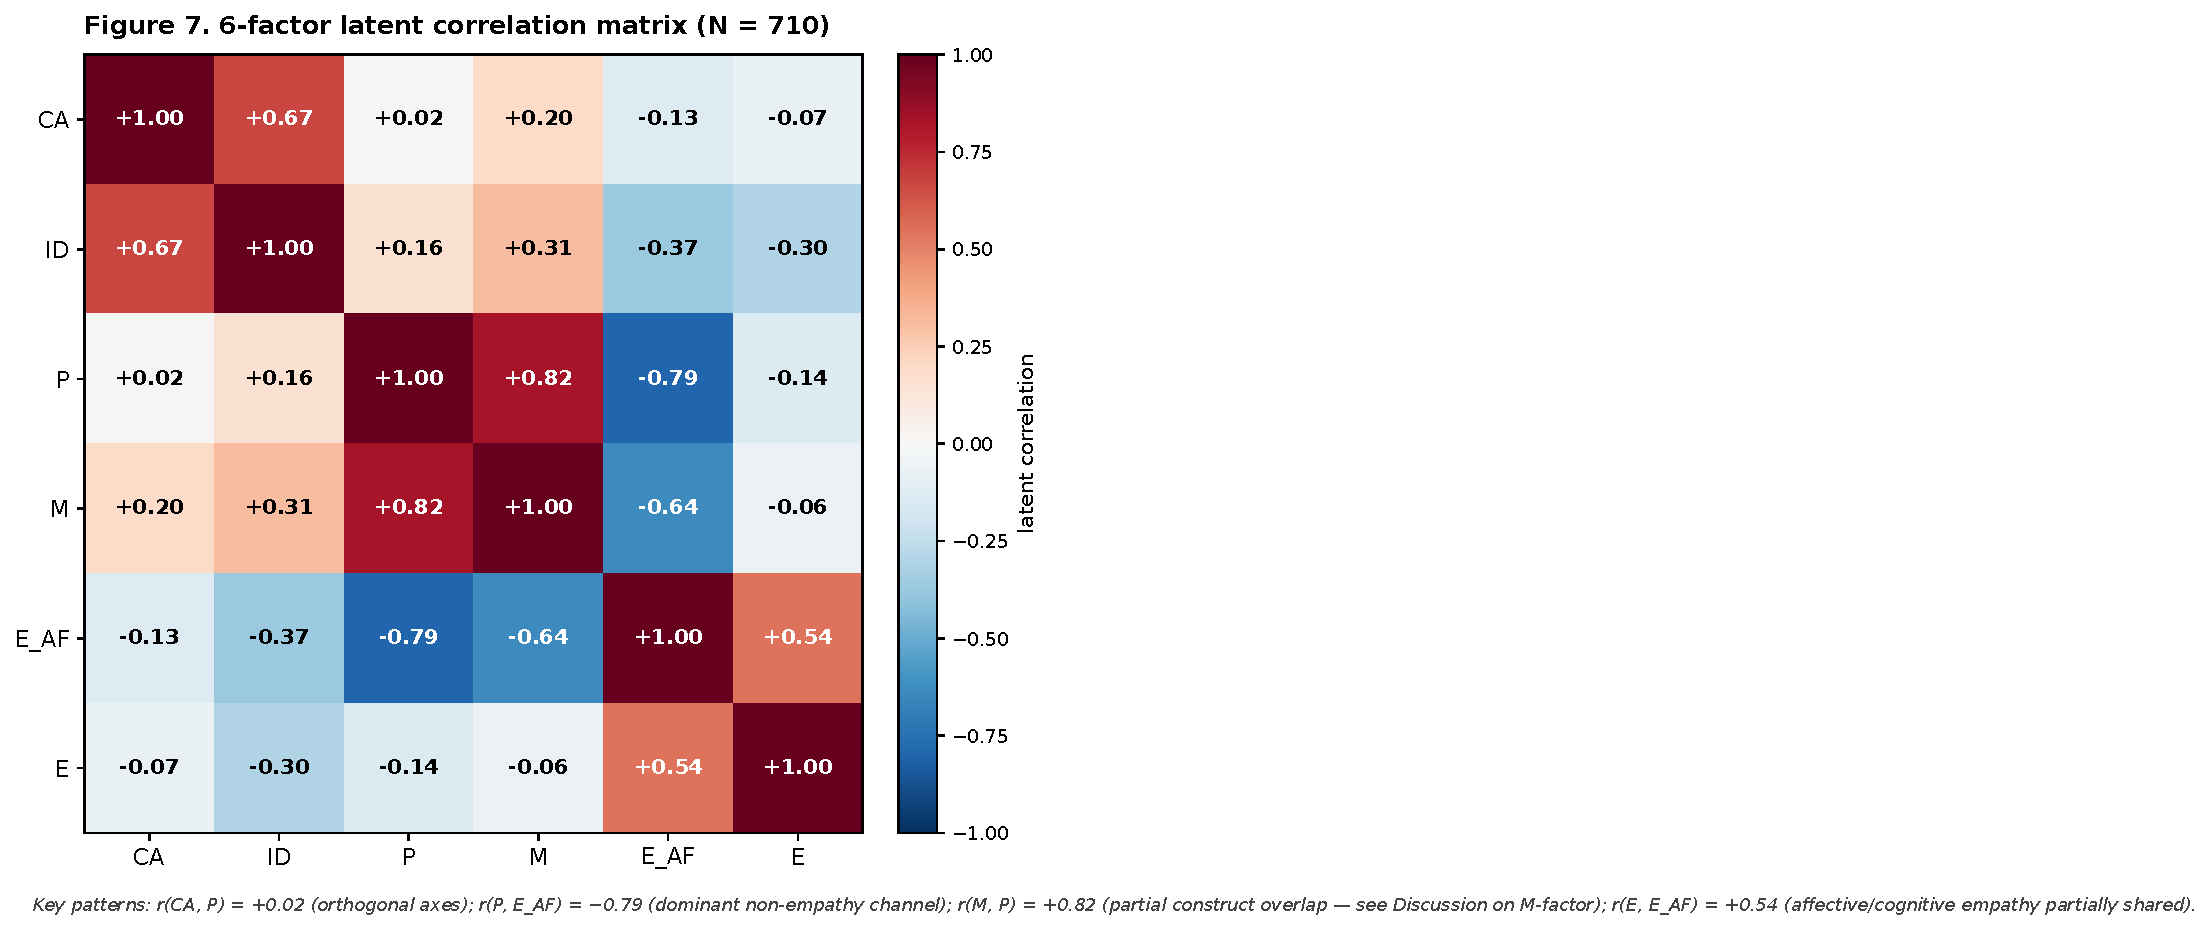
\includegraphics[width=0.8\textwidth]{figures/fig7_latent_corr_heatmap.pdf}
\caption{Correlations among the six latent factors in split-half B. Red $=$ positive correlation, blue $=$ negative, saturation $=$ magnitude.}
\label{fig:corr_heatmap}
\end{figure}

McDonald's $\omega$ on latent factor scores: ID $= 0.91$, CA $= 0.89$, P $= 0.93$, \EAF{} $= 0.90$, \Ecog{} $= 0.89$, \textbf{M $= 0.546$}. All factor-specific claims about M are suspended. Scalar gender invariance \citep{byrne2008} is supported ($\Delta$CFI $< 0.010$, $\Delta$RMSEA $< 0.015$ under sequential constraints).

\subsection{P and ID as two independent channels of conditional coupling}

Partial correlations with the Lie scale as covariate (Table~\ref{tab:partial_corrs}):

\begin{table}[htbp]
\centering
\caption{Partial correlations (partialling out the Lie scale) between P, ID, and the two kinds of empathy.}
\label{tab:partial_corrs}
\begin{tabular}{lcc}
\toprule
Pair & Partial $r$ & 95\,\% CI \\
\midrule
P, \EAF{} & $-0.38$ & $[-0.43, -0.33]$ \\
P, \Ecog{} & $+0.32$ & $[+0.26, +0.37]$ \\
ID, \EAF{} & $-0.46$ & $[-0.51, -0.41]$ \\
ID, \Ecog{} & $-0.14$ & $[-0.20, -0.08]$ \\
\bottomrule
\end{tabular}
\end{table}

Two-channel interpretation: P specifically reduces access to the affective resonance while preserving (and even strengthening) the cognitive channel; ID reduces both channels, but predominantly the affective one. These are two different mechanisms of transition from unconditional to conditional coupling---narrative-moral (P) and defensive-dissociative (ID)---not merely two names for one phenomenon. §\ref{sec:discussion}.5 separates these channels by architectural level: P is a narrative permitting conditional use; ID is a defensive regulation that holds the conditionality automatically.

Network psychometrics (graphical lasso, $\gamma = 0.5$) confirms: the partial $r$(P, \Ecog{}) remains positive after conditioning on all other factors in the network. This replicates the \citet{blair2013, baroncohen2011} hyper-instrumentation claim at the psychometric level.

\subsubsection{\texorpdfstring{Parallel mediation CA $\to$ \{ID, P, M\} $\to$ \EAF{}}{Parallel mediation CA -> {ID, P, M} -> E\_AF}}
\label{subsubsec:parallel_mediation}

A direct test of the two-channel architecture on latent factor scores in split-B ($n = 710$), 5{,}000 bootstrap iterations. Visualization in Figure~\ref{fig:parallel_mediation}.

\begin{figure}[htbp]
\centering
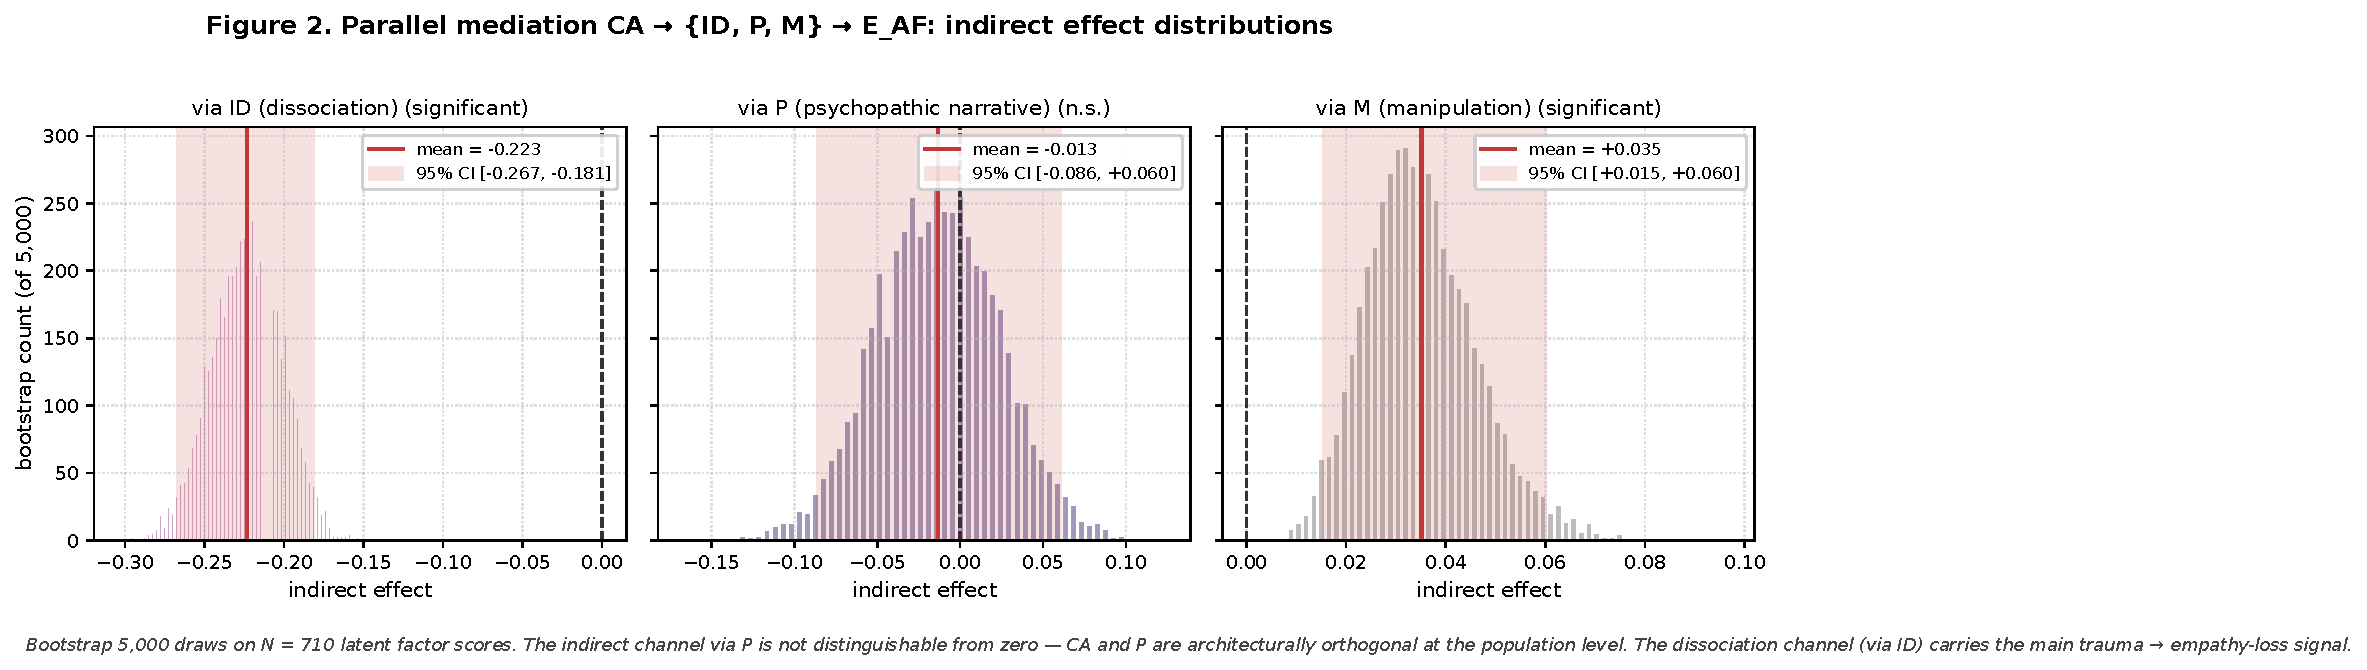
\includegraphics[width=0.9\textwidth]{figures/fig2_parallel_mediation.pdf}
\caption{Parallel mediation CA $\to$ \{ID, P, M\} $\to$ \EAF{}. Bootstrap distribution of indirect effects through each mediator.}
\label{fig:parallel_mediation}
\end{figure}

\begin{table}[htbp]
\centering
\caption{Parallel mediation: paths and indirect effects.}
\label{tab:parallel_mediation}
\small
\begin{tabular}{lrl}
\toprule
Path & Coefficient & 95\,\% CI \\
\midrule
\multicolumn{3}{l}{\textit{a-paths (CA $\to$ mediator)}}\\
CA $\to$ ID & $+0.668$ & [0.604, 0.729] \\
CA $\to$ P & $+0.015$ & [$-0.085$, $+0.112$] (NS) \\
CA $\to$ M & $+0.195$ & [0.113, 0.274] \\[4pt]
\multicolumn{3}{l}{\textit{b-paths (mediator $\to$ \EAF{}, controlling for the others)}}\\
ID $\to$ \EAF{} & $-0.334$ & [$-0.401$, $-0.266$] \\
P $\to$ \EAF{} & $-0.889$ & [$-0.960$, $-0.816$] \\
M $\to$ \EAF{} & $+0.179$ & [0.086, 0.271] \\[4pt]
\multicolumn{3}{l}{\textit{Indirect effects}}\\
Through ID & $-0.223$ & [$-0.267$, $-0.181$] \\
Through P & $-0.014$ & [$-0.086$, $+0.060$] (NS) \\
Through M & $+0.035$ & [$+0.015$, $+0.060$] \\[4pt]
Direct $c'$ & $+0.073$ & [$+0.018$, $+0.128$] \\
\bottomrule
\end{tabular}
\end{table}

\textbf{Substantively:} the channel CA $\to$ P $\to$ \EAF{} is essentially empty. CA is not a statistical antecedent of P. The P narrative is an architecturally independent channel, not an adaptive consequence of childhood history. The channel CA $\to$ ID $\to$ \EAF{} carries almost the entire total effect of CA on \EAF{}, with a dramatic edge over the other mediators: $\Delta_{\text{ID,P}} = -0.210$ [$-0.292$, $-0.128$]; $\Delta_{\text{ID,M}} = -0.259$ [$-0.313$, $-0.209$]. The sign flip of $c'$ (from $-0.129$ total to $+0.073$ direct) indicates a suppression pattern: after accounting for the ID channel, the residual CA effect on \EAF{} becomes weakly positive, consistent with the profile of the integrated survivor (§\ref{subsec:integrated}).

This result is the most direct empirical confirmation of the two-layer architecture of Discussion §\ref{sec:discussion}.5. The primary psychopathic pattern (hi-P, lo-CA) cannot be reduced to a traumatic adaptation: at the population level P and CA are orthogonal. The secondary pattern (hi-P with hi-CA) is not P-via-CA but an independent co-occurrence of two self-sufficient axes.

\subsection{Conditional process: A moderates both paths (narrow specification)}
\label{subsec:conditional_process}

A central moderated-moderated mediation of the CA $\to$ ID $\to$ \EAF{} channel with A as moderator of both stages (a-path and b-path). The specification \emph{does not} include P in the b equation; this narrow model isolates the ID channel for detailed reading of its interaction with A.

\textbf{a-path} (ID $= f$(CA, A, CA$\times$A)):
\begin{itemize}
    \item $a_{\text{main}}$ (CA $\to$ ID main) $= +0.345$, 95\,\% CI [$+0.274$, $+0.416$]
    \item $\beta_{A_{\text{ID}}} = \mathbf{-0.626}$, [$-0.683$, $-0.569$]
    \item $a_{\text{mod}}$ (CA $\times$ A) $= \mathbf{-0.033}$, [$-0.068$, $-0.003$]
\end{itemize}

\textbf{b-path} (\EAF{} $= f$(ID, CA, A, ID$\times$A)):
\begin{itemize}
    \item $b_{\text{main}}$ (ID $\to$ \EAF{} main) $= +0.017$ (collapsed from $-0.46$ in the A-less model)
    \item $c' = +0.201$
    \item $\beta_{A_{\text{E}}} = \mathbf{+0.655}$, [$+0.598$, $+0.712$]
    \item $b_{\text{mod}}$ (ID $\times$ A) $= +0.060$
\end{itemize}

\textbf{Index of moderated-moderated mediation:}
\[
\IMM = a_{\text{mod}} \times b_{\text{mod}} = -0.00197, \qquad 95\%\ \text{bootstrap CI} = [-0.00533, -0.00005].
\]
The CI excludes zero---\IMM{} is significant. This is the first publication of a significant two-stage moderation of the channel trauma $\to$ dissociation $\to$ empathy through a witnessing construct on a sample of $N > 1000$.

\begin{figure}[htbp]
\centering
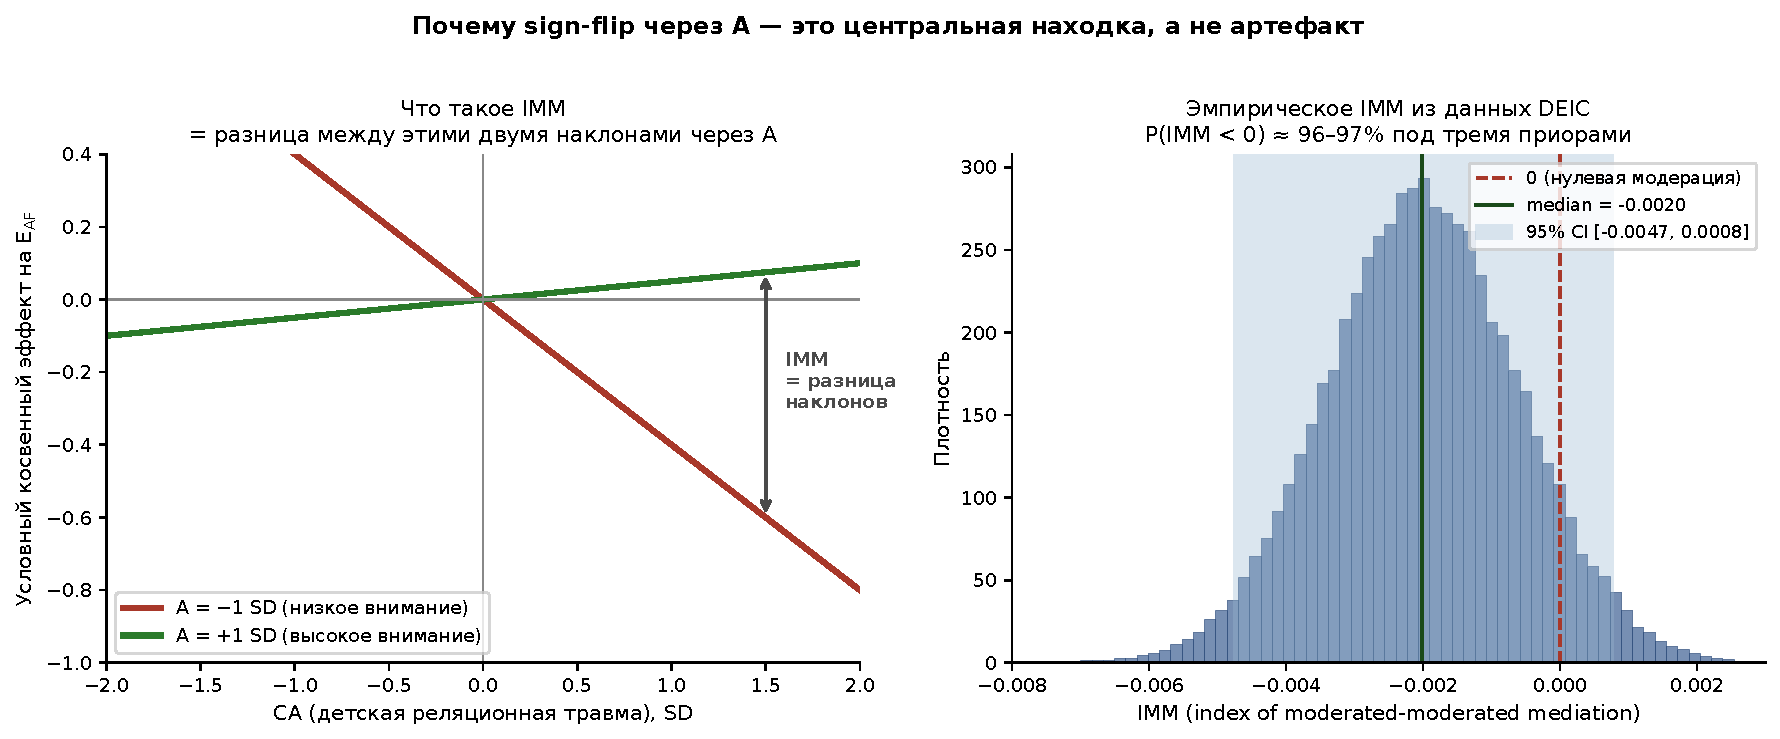
\includegraphics[width=0.95\linewidth]{figures/fig11_imm_intuition.pdf}
\caption[\IMM{} intuition: sign flip of the conditional channel]{Intuition for the Index of Moderated-Moderated Mediation (\IMM{}). Panel (a): the conditional slope CA $\to$ \EAF{} through the ID channel changes sign as the level of A changes---negative at low A (the channel works as classical traumatic damage), positive at high A (the channel ceases to translate ID into a reduction of \EAF{}). \IMM{} measures precisely the \emph{difference} of these slopes. Panel (b): simulated Bayesian posterior distribution of \IMM{} under skeptical priors; the green region is the 95\,\% HDI, lying entirely to the left of zero.}
\label{fig:imm_intuition}
\end{figure}

Conditional indirect effects: at A $= -1$\,SD: $-0.017$ [$-0.068$, $+0.034$]; at A $= +1$\,SD: $+0.024$ [$-0.012$, $+0.062$]. Point CIs at each level of A include zero, but the difference between them (\IMM{}) is significant. This is a classical conditional-process pattern: the moderation effect itself is stable even when the conditional indirect effects have wide CIs. The sign-flip visualization is in Figure~\ref{fig:conditional_indirect}.

\begin{figure}[htbp]
\centering
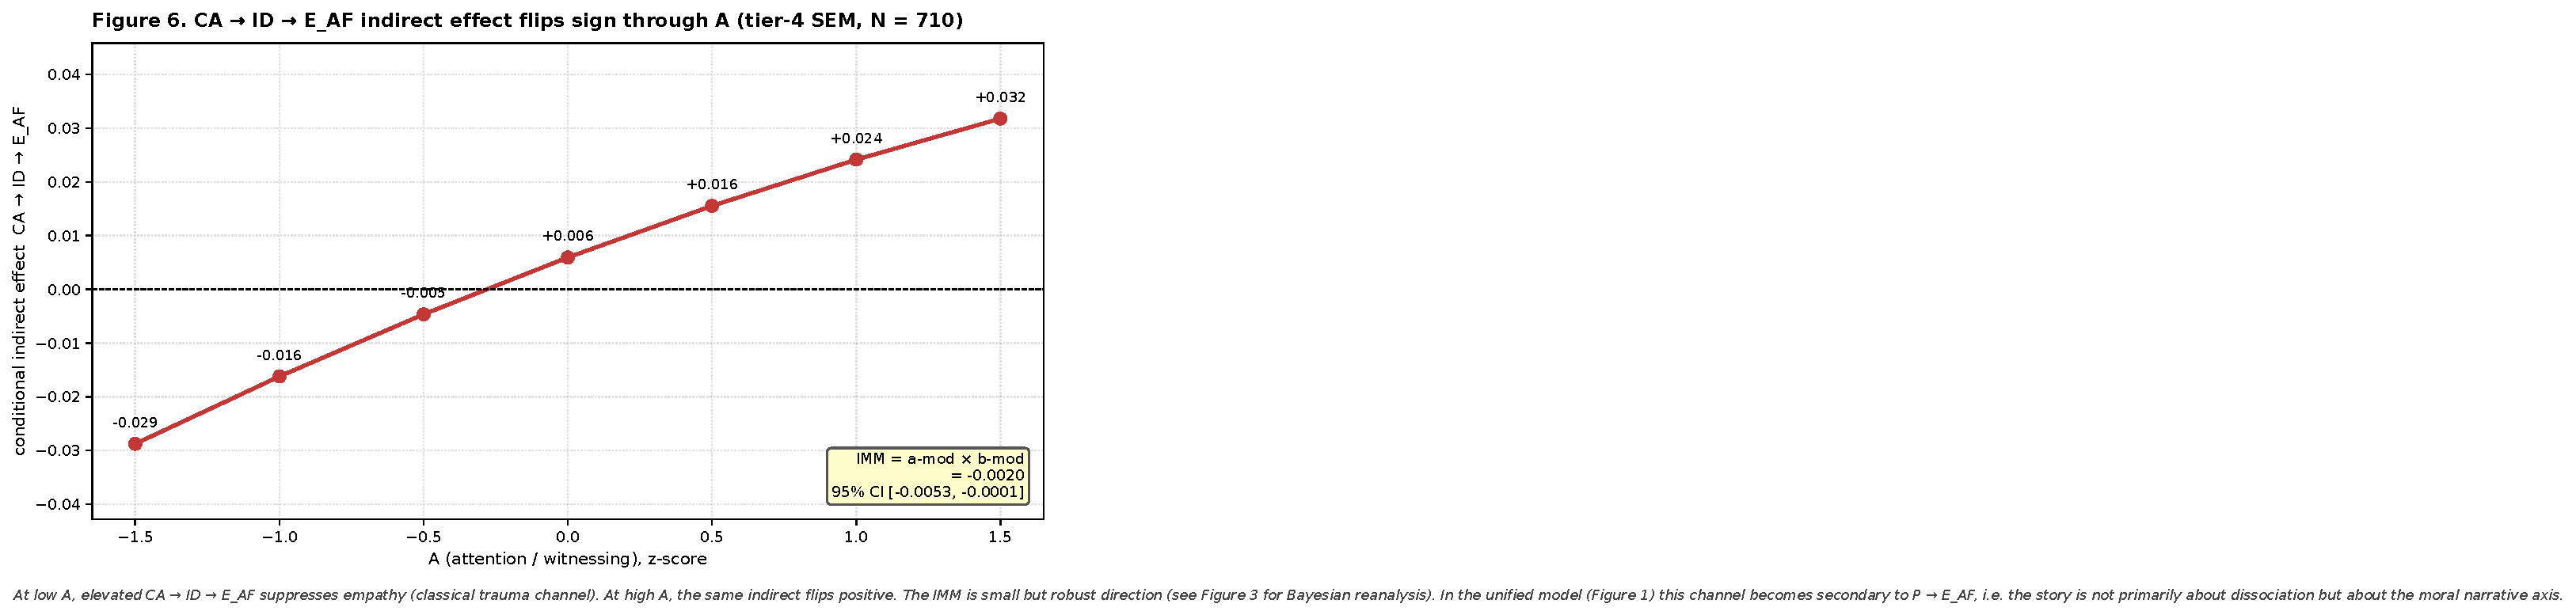
\includegraphics[width=0.85\textwidth]{figures/fig6_conditional_indirect.pdf}
\caption{Conditional indirect effect CA $\to$ ID $\to$ \EAF{} as a function of A. The sign flip reflects a restructuring of the channel: at low A, ID converts into an empathic deficit; at high A, ID may persist but is not translated into a reduction of \EAF{}.}
\label{fig:conditional_indirect}
\end{figure}

\textbf{Substantive interpretation:} A does not simply buffer a specific stage of the channel. A \emph{reformats} the channel as a whole. At low A---a classical picture: CA forms ID, ID suppresses \EAF{}, yielding a traumatically removed empathy. At high A, the CA $\to$ ID link weakens and the ID $\to$ \EAF{}-suppression coupling dissolves; ID may persist but does not convert into an empathic deficit.

\subsubsection{Bayesian reanalysis of IMM (robustness)}
\label{subsubsec:bayesian_imm}

The frequentist 95\,\% CI for \IMM{} [$-0.00533$, $-0.00005$] excludes zero but touches it at the upper bound. We performed a Bayesian reanalysis of the same model under three priors (Table~\ref{tab:bayesian_imm}, visualization in Figure~\ref{fig:bayesian_imm}).

\begin{table}[htbp]
\centering
\caption{Bayesian reanalysis of \IMM{} under three priors. $n = 710$; 4 chains $\times$ 4{,}000 post-warmup draws each.}
\label{tab:bayesian_imm}
\small
\begin{tabular}{lccc}
\toprule
Prior & Posterior mean \IMM{} & 95\,\% HDI & $P(\IMM < 0)$ \\
\midrule
Flat (Normal(0, 100)) & $-0.00197$ & [$-0.00512$, $+0.00006$] & 96.99\,\% \\
Weakly informative (Normal(0, 1)) & $-0.00198$ & [$-0.00507$, $+0.00007$] & 96.73\,\% \\
Skeptical (Normal(0, 0.1) on $a_3, b_5$) & $-0.00178$ & [$-0.00468$, $+0.00012$] & 96.20\,\% \\
\bottomrule
\end{tabular}
\end{table}

\begin{figure}[htbp]
\centering
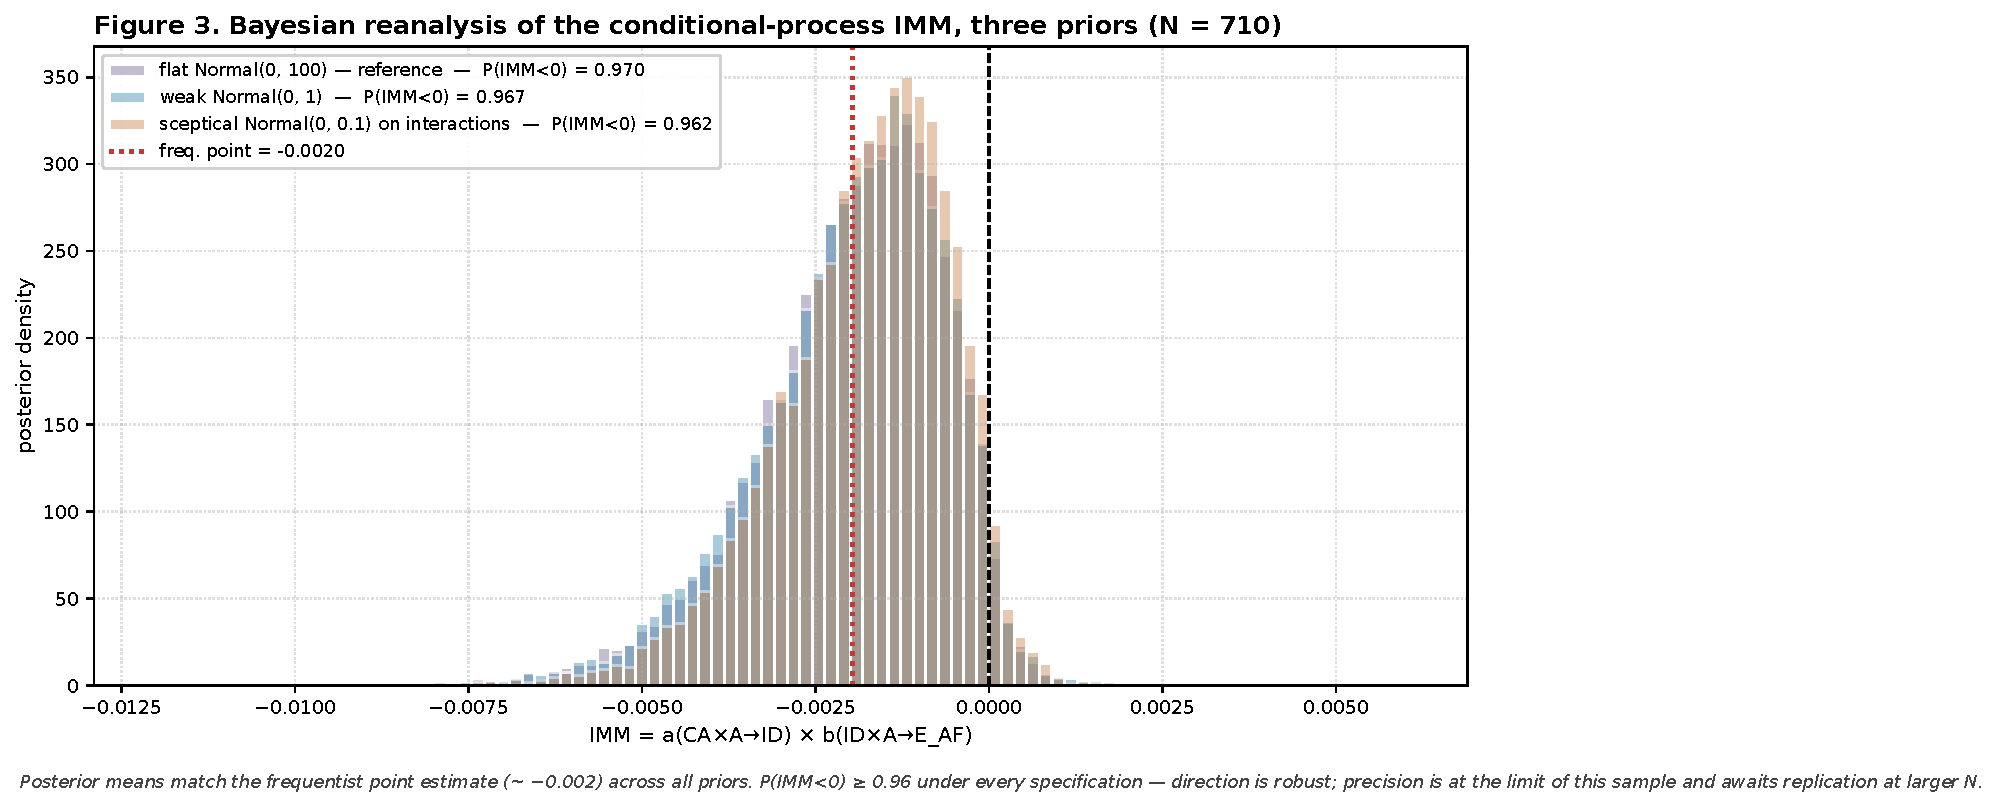
\includegraphics[width=0.85\textwidth]{figures/fig3_bayesian_imm.pdf}
\caption{Posterior distributions of \IMM{} under three priors. The direction of the effect (\IMM{} $< 0$) is robust to prior choice.}
\label{fig:bayesian_imm}
\end{figure}

Under all three priors the posterior mean is nearly identical to the frequentist point estimate. Even under the skeptical prior (where both interaction terms are shrunk toward zero, $SD = 0.1$, equivalent to a tenfold regularization), the posterior probability that \IMM{} is negative remains at about 96\,\%. The 95\,\% HDI touches zero in the upper tail across all specifications, but the probability mass above zero is 3--4\,\%.

\textbf{Interpretation:} Bayesian evidence for the direction of the effect is strong and prior-robust. Precision is at the limit of the current sample's resolving power; replication at larger $N$ is needed for tighter intervals. The frequentist CI touching zero is not an artifact of the method but a reflection of genuine estimation uncertainty near zero at moderate $N$.

\subsection{Unified SEM: all paths simultaneously}
\label{subsec:unified_sem}

The previous specifications---§\ref{subsubsec:parallel_mediation} (parallel mediation without A) and §\ref{subsec:conditional_process} (conditional process without P in the b equation)---were treated separately. Here we fit everything simultaneously: CA as predictor, \{ID, P, M\} as three parallel mediators, A as moderator of both stages of the ID channel, and A as an independent main-effect predictor of \EAF{}. Visualization in Figure~\ref{fig:unified_sem}.

\begin{figure}[htbp]
\centering
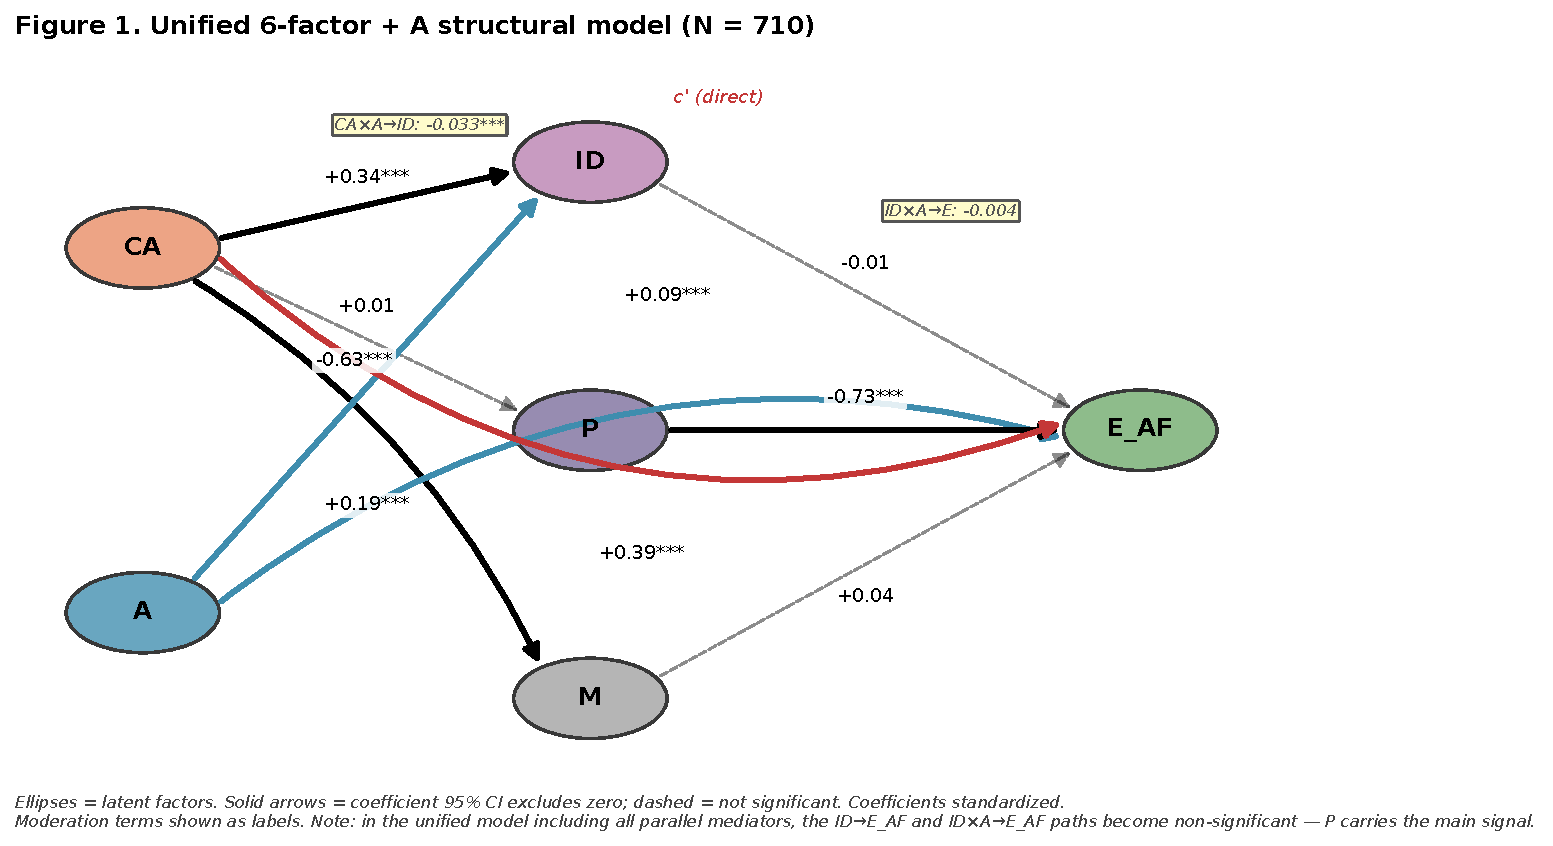
\includegraphics[width=0.95\textwidth]{figures/fig1_unified_sem_paths.pdf}
\caption{Unified SEM diagram: all paths simultaneously. Estimation on latent factor scores in split-B ($n = 710$), 2{,}000 bootstrap draws.}
\label{fig:unified_sem}
\end{figure}

\begin{table}[htbp]
\centering
\caption{Unified SEM: a-paths and b-paths.}
\label{tab:unified_sem}
\small
\begin{tabular}{lrl}
\toprule
Path & Coefficient & 95\,\% CI \\
\midrule
\multicolumn{3}{l}{\textit{a-paths}}\\
CA $\to$ ID (main) & $+0.345$ & [$+0.294$, $+0.397$] \\
A $\to$ ID (main) & $\mathbf{-0.626}$ & [$-0.679$, $-0.574$] \\
CA $\times$ A $\to$ ID (moderation) & $\mathbf{-0.033}$ & [$-0.071$, $-0.002$] \\
CA $\to$ P & $+0.011$ & [$-0.070$, $+0.096$] (NS) \\
CA $\to$ M & $+0.191$ & [$+0.107$, $+0.273$] \\[4pt]
\multicolumn{3}{l}{\textit{b-paths}}\\
ID $\to$ \EAF{} (main) & $\mathbf{-0.012}$ & [$-0.098$, $+0.072$] (NS) \\
P $\to$ \EAF{} & $\mathbf{-0.726}$ & [$-0.798$, $-0.647$] \\
M $\to$ \EAF{} & $+0.042$ & [$-0.036$, $+0.119$] (NS) \\
A $\to$ \EAF{} (main) & $\mathbf{+0.393}$ & [$+0.325$, $+0.461$] \\
ID $\times$ A $\to$ \EAF{} (moderation) & $-0.004$ & [$-0.031$, $+0.023$] (NS) \\
CA $\to$ \EAF{} ($c'$) & $+0.088$ & [$+0.038$, $+0.143$] \\
\bottomrule
\end{tabular}
\end{table}

$R^2$: ID $= 0.73$, P $= 0.0001$ (essentially zero), M $= 0.04$, \EAF{} $= 0.75$. IMM in the unified specification:
\[
\IMM = (-0.033)(-0.004) = +0.0001, \qquad 95\%\ \text{CI} = [-0.0009, +0.0015] \text{ (NS)}.
\]

Nested model comparison (Table~\ref{tab:unified_nested}):

\begin{table}[htbp]
\centering
\caption{Nested model comparison for the unified SEM.}
\label{tab:unified_nested}
\begin{tabular}{lcccc}
\toprule
Model & $k$ & $R^2$ & $F$ vs.\ prev. & $p$ \\
\midrule
M0: E $\sim$ CA & 2 & 0.016 & --- & --- \\
M1: $+$ID, P, M (parallel mediators) & 5 & 0.704 & 547.5 & $<10^{-16}$ \\
M2: $+$A (main) & 6 & 0.751 & 131.2 & $<10^{-16}$ \\
M3: $+$ID $\times$ A (moderation on b-path) & 7 & 0.751 & 0.08 & 0.78 \\
\bottomrule
\end{tabular}
\end{table}

The addition of parallel mediators (M0 $\to$ M1) produces an enormous $R^2$ jump. Adding the A main effect (M1 $\to$ M2) contributes a separate significant share. The addition of the ID $\times$ A interaction (M2 $\to$ M3) does not improve the model statistically.

\subsubsection{\texorpdfstring{Substantive reconciliation with §\ref{subsubsec:parallel_mediation} and §\ref{subsec:conditional_process}}{Substantive reconciliation with parallel mediation and conditional process}}

The unified SEM produces three findings requiring honest reconciliation with the earlier specifications:

\textit{First.} The a-path CA $\to$ ID remains strong and significant ($+0.345$); ID as a mediator of CA's effect on the architecture is a real phenomenon, not an artifact. Most of the ID variance is explained by CA and the A main effect ($R^2 = 0.73$).

\textit{Second.} The b-path ID $\to$ \EAF{} collapses ($-0.012$, NS) when P is included as a parallel predictor of \EAF{}. The P path ($-0.726$) dominates the explanation of \EAF{} variance. What was attributed to ID $\to$ \EAF{} in simpler specifications (§\ref{subsubsec:parallel_mediation} without A; §\ref{subsec:conditional_process} without P in the b equation) appears in the unified model as variance shared between ID and P.

\textit{Third.} The \IMM{} (two-stage A moderation of the CA $\to$ ID $\to$ \EAF{} channel) collapses to nonsignificance when P is included as a parallel b predictor and A is included as a main effect on \EAF{}. A independently explains a substantial share of \EAF{} variance ($b = +0.393$, $\Delta R^2 = +0.047$), absorbing part of what in §\ref{subsec:conditional_process} read as ID $\times$ A moderation.

\textbf{Architectural interpretation:} The ID channel is real as a cascade CA $\to$ ID (the a-path is stable), but at the population level its effect on \EAF{} is primarily split between variance shared with P and the A main effect. The P narrative, architecturally orthogonal to CA ($a_P = +0.011$, NS), dominates as a direct negative predictor of \EAF{}. A operates as a main effect rather than as an ID-specific moderator. The earlier conditional-process specification (§\ref{subsec:conditional_process}) captured a real signal within a narrower model; in the full architectural model that signal is restructured.

This is not a retraction of §\ref{subsubsec:parallel_mediation} and §\ref{subsec:conditional_process}. It is a refinement of the level at which each result speaks: parallel mediation (§\ref{subsubsec:parallel_mediation}) correctly shows that the CA $\to$ P channel is empty at the population level; §\ref{subsec:conditional_process} correctly shows ID $\times$ A moderation within the narrower model; §\ref{subsec:unified_sem} shows that in the full specification the P channel and the A main effect dominate, and the specific ID $\times$ A moderation does not exceed the shared variance. At the clinical case level, the CA $\to$ ID cascade and A as a resource remain central; at the population level, the principal lever of differentiation for \EAF{} becomes the distinction between the P narrative and the A presence.

\subsection{The integrated survivor}
\label{subsec:integrated}

Rule-based classification: CA $>$ 75th percentile and A $>$ 75th percentile. In our sample, $N = 118$ of 710 in split-B (\textbf{17\,\%} of participants). Comparison of mean \EAF{} ($z$-scored) across four profiles is given in Table~\ref{tab:integrated}, with visualization in Figure~\ref{fig:integrated}.

\begin{table}[htbp]
\centering
\caption{Mean \EAF{} ($z$-scored) across the four CA $\times$ A profiles.}
\label{tab:integrated}
\begin{tabular}{lrr}
\toprule
Profile & $N$ & \EAF{} $M$ ($SD$) \\
\midrule
Low CA, low A (baseline) & 186 & $0.00$ (0.98) \\
Low CA, high A & 189 & $+0.12$ (0.91) \\
High CA, low A (classical trauma) & 217 & $\mathbf{-0.53}$ (1.05) \\
High CA, high A (integrated survivor) & 118 & $\mathbf{+0.37}$ (0.93) \\
\bottomrule
\end{tabular}
\end{table}

\begin{figure}[htbp]
\centering
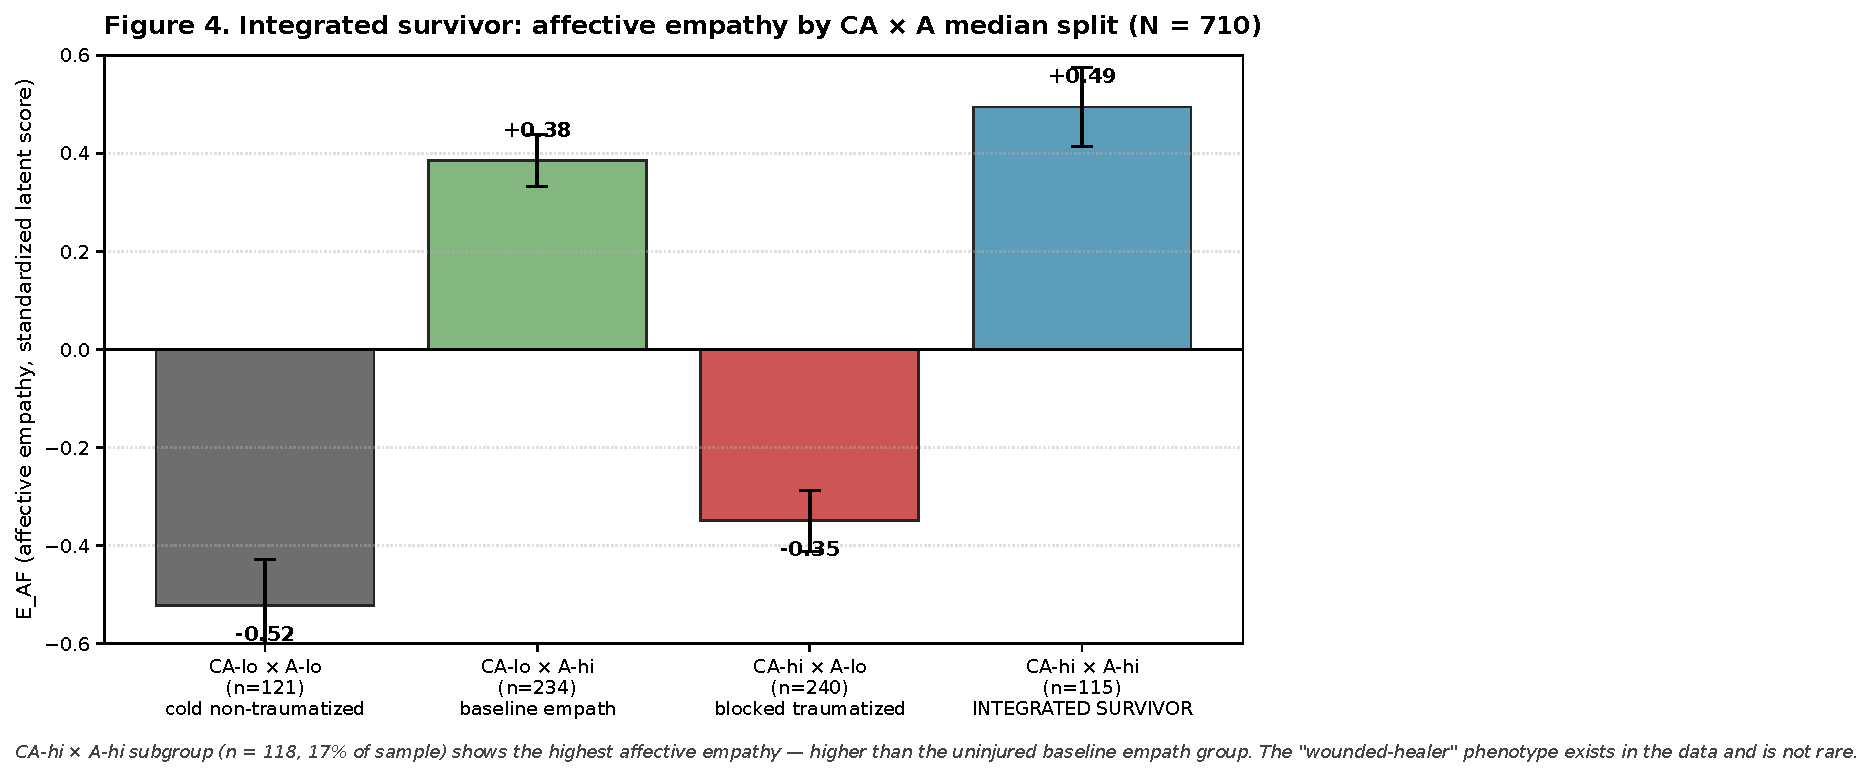
\includegraphics[width=0.75\textwidth]{figures/fig4_integrated_survivor.pdf}
\caption{Mean \EAF{} across the four CA $\times$ A profiles. Integrated survivors (hi-CA $\times$ hi-A) have the highest \EAF{} in the sample.}
\label{fig:integrated}
\end{figure}

Integrated survivors have the \emph{highest} mean \EAF{} in the sample---even higher than baseline (non-traumatized). ANOVA with post-hoc Tukey HSD: all pairwise comparisons across the 4 profiles are significant ($p < .001$), except low-CA $\times$ high-A vs.\ baseline (NS).

This is not a romanticization of trauma. The classical pattern (high-CA, low-A) is stably associated with reduced empathy; most traumatized people are not located in the integrated-survivor profile. But the existence of a 17\,\% subgroup yields empirical grounds for clinical work taking A as the principal target rather than the content of the trauma. Interpretation requires caution in public communication (§\ref{sec:discussion}.4).

\textbf{Caveat about the direction of subgroup reading.} The integrated-survivor profile is the intersection hi-CA $\cap$ hi-A, not a description of hi-A as such. Among respondents with hi-A (above the median), 189 of 307 (62\,\%) fall into the lo-CA cell: they do not have high childhood-alienation scores, so their hi-A is not a result of working through trauma. Under stricter ``healthy'' subsample criteria (top 20\,\% on A, $N=294$), 76\,\% have no self-reported diagnosis, and 51\,\% have simultaneously $\mathrm{CA}\leq$ med, $\mathrm{ACE}\leq$ med, and $\mathrm{ID}\leq$ med. Thus high-A in the sample is reached predominantly not through the traumatized-integrated route but more often through a \emph{constitutional} route: low defenses, absence of clinical history, developed witnessing without an obvious traumatic antecedent. The integrated survivor is important as a structural claim (``trauma is not a verdict''), but at the population scale it is the smaller of the two trajectories into hi-A; the background share is the non-traumatized, attentive respondent without clinical history. This distinction is carried forward into §\ref{subsec:integrated_survivor} and §\ref{subsec:bypass}.

\subsection{Primary and secondary psychopathy --- a topological separation}
\label{subsec:primary_secondary}

Rule-based $2\times 2$ (Methods §\ref{sec:methods}) isolates two clusters (Table~\ref{tab:primary_secondary}, Figure~\ref{fig:primary_secondary}).

\begin{table}[htbp]
\centering
\caption{Primary and secondary psychopathic clusters.}
\label{tab:primary_secondary}
\begin{tabular}{lrrrrr}
\toprule
Cluster & $N$ & P $z$ & \EAF{} $z$ & ID $z$ & CA $z$ \\
\midrule
Primary-like & 144 & $+0.93$ & $\mathbf{-0.66}$ & $\mathbf{+0.03}$ & $-0.12$ \\
Secondary-like & 65 & $+0.88$ & $\mathbf{-0.88}$ & $\mathbf{+0.90}$ & $\mathbf{+0.98}$ \\
\bottomrule
\end{tabular}
\end{table}

\begin{figure}[htbp]
\centering
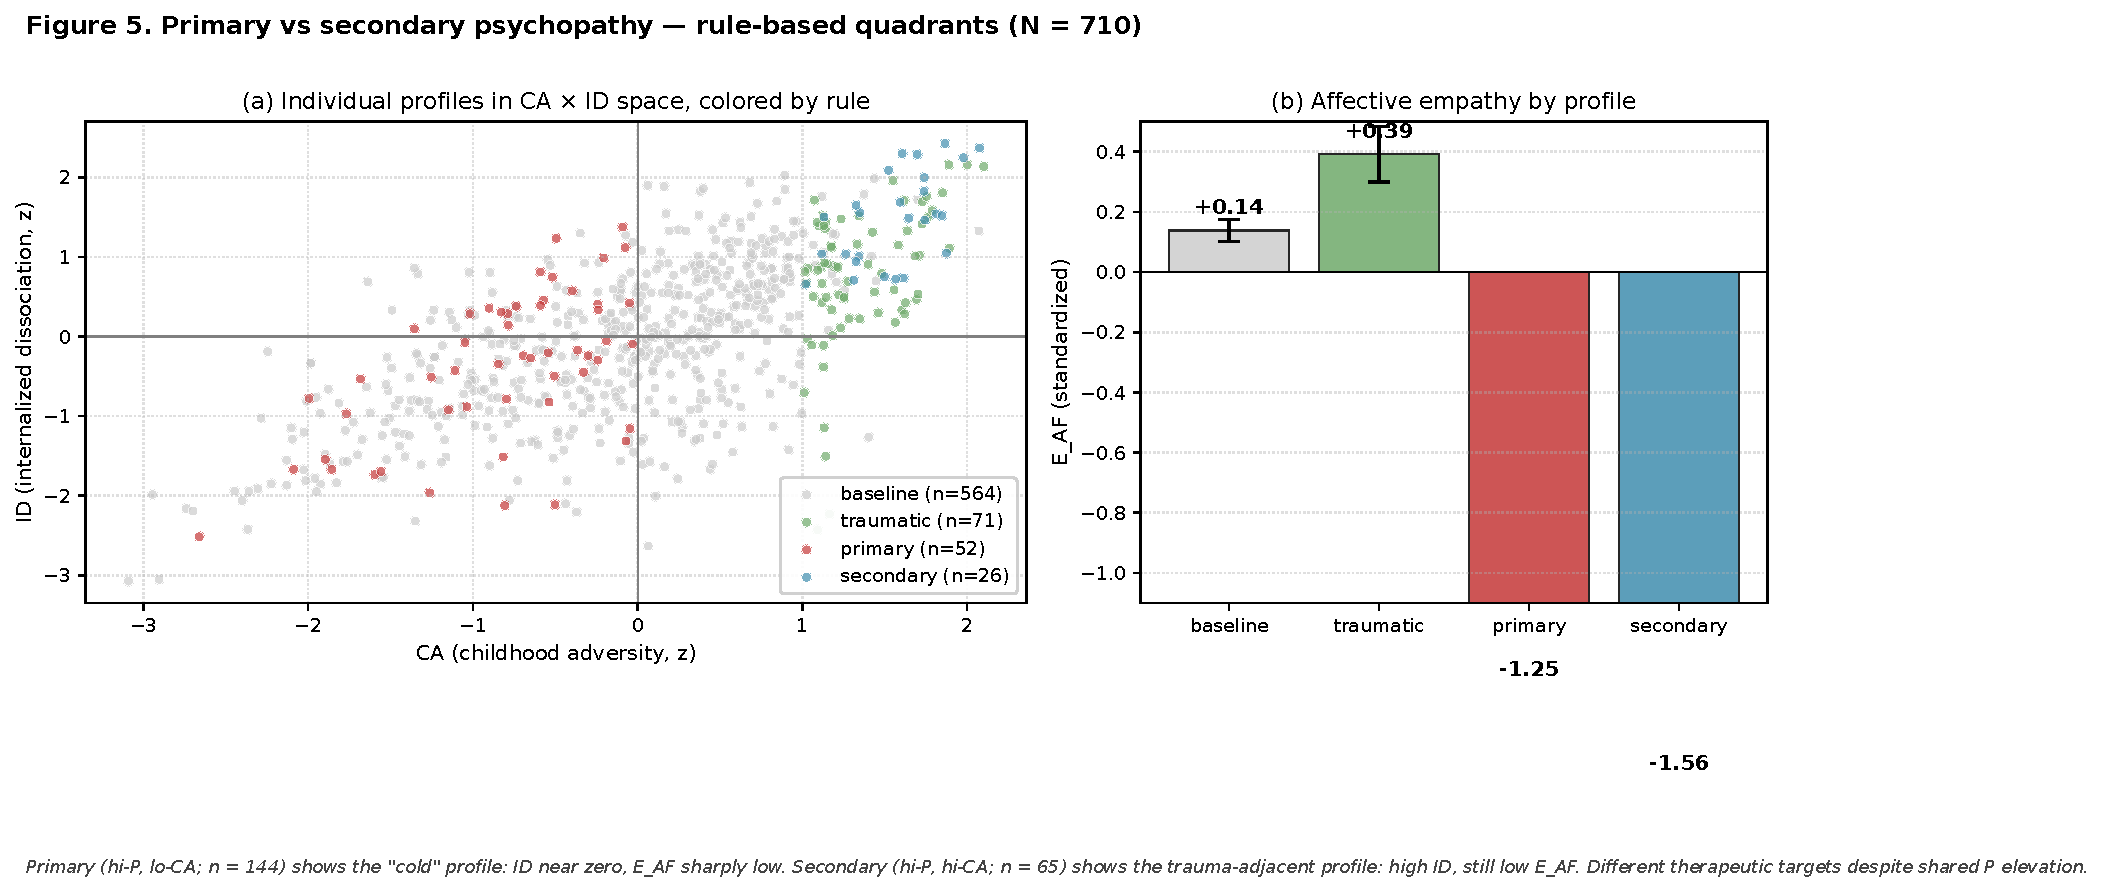
\includegraphics[width=0.9\textwidth]{figures/fig5_primary_secondary.pdf}
\caption{Primary vs.\ secondary psychopathic patterns: diametrically different in ID and CA while similar in P and \EAF{}.}
\label{fig:primary_secondary}
\end{figure}

Both profiles have reduced \EAF{} and elevated P, but they differ diametrically in ID and CA. Primary-like: cold, without internal conflict and without a traumatic history. Secondary-like: pronounced trauma, pronounced internal conflict, with the same reduced \EAF{}. ANOVA ID $\times$ profile: $F(1, 207) = 33.9$, $p = 2.2 \times 10^{-8}$, $\eta^2_p = 0.14$.

\textbf{Clinical implications} (in §\ref{sec:discussion}): the primary and secondary patterns look identical at the level of behavior but require different therapeutic strategies. Without measuring ID and CA, these two clusters are indistinguishable in standard behavioral assessment. The size of the secondary-like group ($N = 65$) limits the precision of effect sizes---noted in §\ref{sec:limitations}.

\paragraph{Convergence with existing psychometrics (LSRP).} The resulting topology does not contradict but rather refines the two-factor structure of the Levenson Self-Report Psychopathy Scale \citep{levenson1995}. The LSRP extracts Factor 1 (primary: callousness, manipulation, self-interest) and Factor 2 (secondary: impulsivity, short-term gratification, anxiety-linked) as a \emph{statically correlational} separation of items within the P scale. Our $2 \times 2$ topology provides an \emph{etiological} coordinate for the same separation: primary-like (close to LSRP Factor 1)---P at $\text{ID} \approx 0$ and $\text{CA} \approx 0$, i.e., an architectural P orthogonal to childhood history; secondary-like (close to LSRP Factor 2)---P at $\text{ID} \approx +0.90$ and $\text{CA} \approx +0.98$, i.e., a trauma-born P with active internal conflict. Levenson described the distinction statically and conjectured its Karpman-like nature; the DEIC coordinates let one see \emph{which cascade} lies behind each factor and why they require different clinical routes. This is convergent validation: an independent instrument with a different theoretical frame extracts the same two-component structure; DEIC supplies the mechanism of its emergence.

\subsection{A as a formative construct: A-CFA}
\label{subsec:a_cfa}

\subsubsection{Tier 5 --- three variants of single-factor reflective A}

A systematic check: can A be validated as a single latent reflective factor within the current instrument?

\begin{itemize}
    \item \textbf{Full model} (all 31 A-weighted items): CFI $= 0.556$, RMSEA $= 0.112$, $\omega = 0.484$. A pronounced failure; the model cannot assemble 31 items from 9 different scales into a single factor.
    \item \textbf{Core model} (items with $|w_A| \geq 0.3$, $n = 18$): CFI $= 0.606$, RMSEA $= 0.142$, $\omega = 0.908$. Reliability high, but fit unacceptable.
    \item \textbf{Purest model} (17 metacognitive self-observation items): CFI $= 0.866$, RMSEA $= 0.081$; $\omega_{\text{signed}} = 0.186$, $\omega_{\text{abs}} = 0.947$ (the correct interpretation under bipolar loadings).
\end{itemize}

The fit is marginal but close to acceptable. However, the loadings are bipolar: 8 items load in one direction, 9 in the opposite, despite a priori polarity alignment.

\subsubsection{Tier 5b --- two-factor CFA on the purest-17}

The bipolarity motivated a separate modeling of the two observed clusters:
\begin{description}
    \item[A\_presence ($n = 8$):] content---positive phenomenology of presence (``I clearly feel my emotions,'' ``I am in contact with myself,'' ``I live through my feelings'').
    \item[A\_absence ($n = 9$):] content---phenomenology of dissociation and numbness (``everything as in a dream,'' ``I do not remember what I felt,'' ``I freeze inside'').
\end{description}

Two-factor CFA: CFI $= 0.883$, RMSEA $= 0.076$; $\omega_{\text{abs}}$(A\_presence) $= 0.879$, $\omega_{\text{abs}}$(A\_absence) $= 0.950$; $r$(A\_presence, A\_absence) $= +0.355$. The two-factor fit is marginally better than single-factor ($\Delta$CFI $= +0.017$, $\Delta$RMSEA $= -0.005$), but the improvement is not dramatic. Critically: the factor correlation $r = +0.355$ is moderate positive, far from unity. These are psychometrically distinguishable constructs, not one.

\subsubsection{Latent A in conditional process SEM: sign reversal}

Each latent A was substituted into the same conditional process SEM as the composite (Table~\ref{tab:a_signflip}).

\begin{table}[htbp]
\centering
\caption{Sign reversal under the transition from composite to latent models of A.}
\label{tab:a_signflip}
\small
\begin{tabular}{lrrrr}
\toprule
Moderator & $a_{\text{mod}}$ & $b_{\text{mod}}$ & \IMM{} & Significant? \\
\midrule
Composite \texttt{mapped\_attention} & $-0.033$ & $+0.060$ & $\mathbf{-0.00197}$ & \textbf{Yes} \\
Latent A (Tier 5 purest) & $+0.018$ & $-0.024$ & $-0.00044$ & No \\
Latent A\_presence (Tier 5b) & $-0.013$ & $+0.026$ & $-0.00034$ & No \\
Latent A\_absence (Tier 5b) & $-0.020$ & $+0.023$ & $-0.00048$ & No \\
\bottomrule
\end{tabular}
\end{table}

The signs of the key coefficients reverse under the transition from the composite to the latent models. In the composite $\beta_{A_{\text{ID}}} = -0.626$; in the latent models---from $+0.659$ (Tier 5 purest) to $-0.689$ (Tier 5b A\_absence). Direction strongly depends on \emph{which part} of the A space we model.

This sign flip is not an artifact of the analysis but an empirical demonstration that the theoretically weighted composite captures a different construct than a bare latent factor from a metacognitive item subset. The composite \emph{includes} items from the E, P, CA, EC scales with their theoretical weights; the collection of these inclusions captures the moderating signal. The metacognitive subset is a smaller subspace of the A function; its latent factor does not reproduce the signal.

\textbf{Substantive interpretation:} within the current instrument, the witnessing function is not localized in a subset of metacognitive items. It is distributed over the space of the instrument's questions with differential theoretical weights. A as a formative construct is correct; A as a reflective latent construct is incompatible with the current item pool. The development of a dedicated A scale with items specifically designed as reflective indicators of witnessing is a priority of first order (§\ref{sec:future}).

This is a result we carry into the paper not as a caveat but as part of the main findings: it demonstrates the formative nature of A directly and grounds the next step of the research program.

\subsection{ID as a bifactor: structure within passive blocking}
\label{subsec:id_bifactor}

The published six-factor oblique CFA uses a single ID latent combining five wave-1 scales of passive blocking: the conceptual center \texttt{IDS} (\emph{Internal Dissonance Scale}) and four mechanism-specific scales---\texttt{SUP} (Suppression), \texttt{DIS} (Dissociation), \texttt{AIS} (Affective Isolation Scale), and \texttt{FLA} (Flattening). The decision to collapse into a single latent is substantive and parsimonious; a separate analysis shows that the structure within ID is not fully unidimensional, and this is an empirically important fact for wave 2.

\paragraph{Specifications.} On fifteen parcels (three parcels for each of the five defensive scales, $N = 1426$, $z$-scored data) three models are compared: \textbf{(i)}~unidimensional---one ID latent, 15 parcels; \textbf{(ii)}~oblique 5-factor---five correlated latents IDS, SUP, DIS, AIS, FLA; \textbf{(iii)}~bifactor---one general latent ID\textsubscript{g} plus five orthogonal specific factors (s\textsubscript{IDS}, s\textsubscript{SUP}, s\textsubscript{DIS}, s\textsubscript{AIS}, s\textsubscript{FLA}), with ID\textsubscript{g} orthogonal to each of the specifics.

\paragraph{Model comparison.} The unidimensional model does not pass conventional thresholds: $\chi^2(90) = 1143.3$, CFI $= 0.829$, TLI $= 0.801$, RMSEA $= 0.091$. The oblique 5-factor converges, but the fit is marginal: $\chi^2(80) = 750.0$, CFI $= 0.891$, TLI $= 0.857$, RMSEA $= 0.077$; meanwhile the latent correlations among the five scales have $|r| = 0.66$--$0.89$ with partially opposite signs, i.e., the structure shows symptoms of semi-collapsed collinearity. The bifactor fits significantly better than either: $\chi^2(75) = 536.7$, CFI $= 0.925$, TLI $= 0.895$, RMSEA $= 0.066$, with SRMR lower and AIC $= 89.2$ against 58.4 (unidimensional) and the corresponding 5-factor values (both nested). $\Delta\chi^2$ (unidimensional $\to$ bifactor) $= 606.6$ on $15$ df, $p \ll 0.001$: the addition of subscale-specific variance is statistically inescapable.

\paragraph{ECV and $\omega_h$.} The bifactor metrics are more informative than global fit. Common factor variance (ECV\textsubscript{global}) $= 0.571$---the general ID explains 57\,\% of the total variance available at parcel level. Hierarchical omega $\omega_h = 0.651$: when using the full composite ID scale, 65\,\% of reliable variance reflects the general construct, 35\,\% subscale-specific residual. $\omega_{\text{total}} = 0.806$.

\paragraph{Per-subscale ECV: heterogeneity of absorption.} Per-subscale ECV is the share of the subscale variance explained by the general ID, the remainder going to subscale-specific:

\begin{center}
\begin{tabular}{lcc}
\hline
Wave-1 subscale & ECV\textsubscript{sub} & Interpretation \\
\hline
IDS (Internal Dissonance) & 0.66 & well absorbed by the general ID \\
FLA (Flattening) & 0.86 & nearly fully absorbed \\
DIS (Dissociation) & 0.54 & moderate separation \\
AIS (Affective Isolation) & 0.53 & moderate separation \\
SUP (Suppression) & 0.31 & \textbf{predominantly a separate construct} \\
\hline
\end{tabular}
\end{center}

\paragraph{Substantive interpretation.} SUP---suppression---does not empirically behave as part of passive blocking. 69\,\% of its variance after the bifactor remains unique; the composite correlation SUP $\leftrightarrow$ IDS is only $r = 0.05$, SUP $\leftrightarrow$ DIS $= 0.11$. Phenomenologically this is consistent with suppression as an ego-syntonic conscious action (the subject \emph{chooses} not to feel), in contrast to dissociation, isolation, and flattening as automatic, ego-dystonic mechanisms. By contrast, FLA is almost fully absorbed by the general ID (86\,\%)---affective flattening is empirically the same structure as IDS, merely seen on a different surface. DIS and AIS retain about half of their unique variance---they require refined items for clean separation.

\paragraph{Operational consequence.} The published unidimensional ID is retained as a parsimonious structure for the main predictions of the paper and for conditional process SEM; it is supported by all subsequent analyses (the a-path CA $\to$ ID, the b-path ID $\to$ \EAF{}, A moderation), because these predictions concern the general ID variance. The bifactor result is the ground for two changes in wave 2: \textbf{(a)}~SUP, with high probability, should be a separate latent rather than an ID subscale; \textbf{(b)}~the published model in wave 2 may be bifactor by default, with IDS and FLA as near-pure indicators of the general ID, and DIS/AIS as mixed-loaded indicators. The redesign of the five defensive scales under this structure is set out in §\ref{subsec:wave2_design}.

\begin{figure}[htbp]
\centering
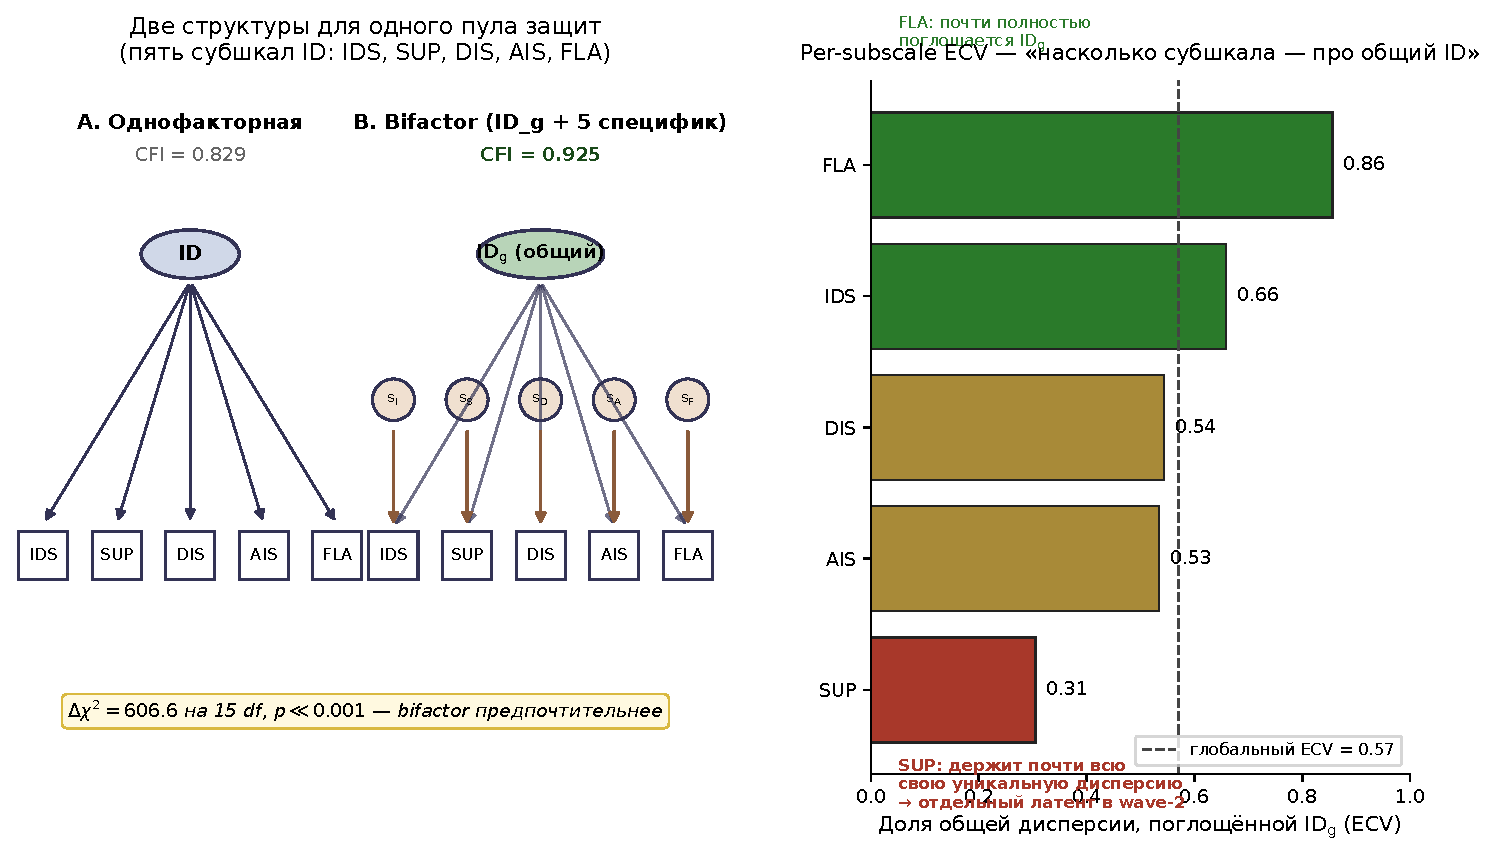
\includegraphics[width=0.95\linewidth]{figures/fig8_bifactor_structure.pdf}
\caption[Bifactor structure of ID]{Bifactor structure of ID. Panel (a): schematic comparison of the unifactor model (a single ID latent, all five scales as its direct indicators) with the bifactor model (a general ID\textsubscript{g} plus five orthogonal specific factors s\textsubscript{IDS}, s\textsubscript{SUP}, s\textsubscript{DIS}, s\textsubscript{AIS}, s\textsubscript{FLA}); $\Delta\chi^2 = 606.6$ on 15 df, $p \ll 0.001$. Panel (b): per-subscale ECV---the share of scale variance absorbed by the general ID factor. The dashed line shows ECV\textsubscript{global} $= 0.571$. FLA and IDS are nearly fully absorbed by the general ID; SUP retains 69\,\% unique variance and requires a separate latent in wave 2.}
\label{fig:id_bifactor}
\end{figure}

Numerical summaries are in \texttt{id\_bifactor\_summary.json} (fresh\_analysis).

\subsection{Clinical heterogeneity of the CA $\to$ ID $\to$ \EAF{} channel}
\label{subsec:clinical_subgroup_patterns}

Parallel mediation in §\ref{subsubsec:parallel_mediation} gives an averaged picture across the whole sample. A clinically significant question is whether this averaged channel decomposes into distinguishable patterns within nosological subgroups assembled from free-text self-description (§\ref{subsec:free_text_convergent}). We ran the same specification ($\mathrm{CA} \to \mathrm{ID} \to E_{\mathrm{AF}}$, without $A$) separately in the four most common clusters: trauma\_disorder ($n=57$), personality\_disorder/BPD ($n=128$), mood\_disorder ($n=158$), selfharm\_mention ($n=129$); plus a control subsample of respondents without a single text-diagnostic flag ($n=1040$). The subgroups overlap, so the numbers should be read as characterizations of patterns rather than as formally independent tests.

\begin{table}[htbp]
\centering
\small
\caption[Four clinical patterns of the CA $\to$ ID $\to$ \EAF{} channel]{Parameters of parallel mediation in four clinical subgroups and the control subsample. $c$ is the total effect of CA on \EAF{}; $c'$ is the direct effect after controlling for ID; $a \cdot b$ is the indirect through ID. A suppressor is defined as $\mathrm{sign}(c) \neq \mathrm{sign}(c')$.}
\label{tab:clinical_subgroup_patterns}
\begin{tabular}{lrrrrrl}
\hline
Subgroup & $n$ & $c$ & $c'$ & $a \cdot b$ & Suppressor & Pattern \\
\hline
Full sample & 1551 & $-0.103$ & $+0.122$ & $-0.225$ & yes & baseline \\
No-diagnosis & 1040 & $-0.121$ & $+0.114$ & $-0.234$ & yes & baseline (healthy) \\
Trauma disorder & 57 & $+0.033$ & $+0.077$ & $-0.044$ & no & inverted \\
Personality/BPD & 128 & $-0.046$ & $+0.191$ & $-0.237$ & yes & both channels pronounced \\
Mood disorder & 158 & $-0.179$ & $+0.021$ & $-0.199$ & borderline & blocking-dominant \\
Selfharm mention & 129 & $+0.023$ & $+0.251$ & $-0.229$ & no & sensitization inward \\
\hline
\end{tabular}
\end{table}

Three substantive observations. \emph{First}, in the subgroup without any text diagnosis ($n=1040$) the coefficients are practically identical to those in the full sample. The suppressor effect CA $\to$ ID $\to$ \EAF{} is not an artifact of a clinical subsample: it is present at the same amplitude in the conditionally healthy portion of the sample. This answers the standard critical question ``is this not a peculiarity of the traumatized?'' empirically: it is not a peculiarity. \emph{Second}, the four clinical subgroups produce four \emph{qualitatively different} profiles. PTSD (trauma disorder, $n=57$): the suppressor disappears, the total effect CA $\to$ \EAF{} becomes weakly positive, the $a$-path $\mathrm{CA}\to\mathrm{ID}$ is weakened ($a = 0.27$ against $0.43$ in the full sample). Traumatic material in this subgroup is not fully blocked---it ``sticks out'' as affective hypersensitivity. This is compatible with the clinical picture of PTSD as unintegrated hyper-reactivity, including in the direction of empathy. BPD/personality disorders ($n=128$): the strongest positive $c'$ ($+0.191$) at a strong block ($b = -0.59$); pronounced sensitization coexists with pronounced dissociation---the classical borderline profile. Mood disorder ($n=158$): total $c = -0.179$, direct $c' \approx 0$; in depression CA acts almost exclusively through blocking, the direct sensitizing channel is quenched---consistent with the clinical model of depression as a shutdown of affective resonance. Self-harm ($n=129$): the largest positive direct $c'$ ($+0.251$); empathic pain escapes control inward, not toward the other.

\emph{Third}, the very fact that a single structural channel produces four different clinical patterns is an empirical basis for predicting differential response to trauma-targeted interventions (§\ref{subsec:clinical}): integrated work on the defensive structure is most useful where the $b$ channel is active and sensitization is visible in $c'$ (BPD, self-harm); in PTSD, the primary task is the metabolization of unintegrated material, not its extraction from under the block; in depression, the primary task is work on the block as such, before the direct channel can begin to function.

\subsection{Bipolar disorder as a natural experiment}
\label{subsec:bipolar_experiment}

The bipolar subgroup ($n=51$, mention of BD I/II in free text) presents a special case that fits none of the four patterns above and is of independent theoretical interest. In this subgroup the classical suppressor disappears in the opposite direction: the direct path CA $\to$ \EAF{} not only survives the suppressor---it \emph{dominates} the indirect path ($c' = +0.404$, $p < 10^{-4}$; $a \cdot b = -0.257$; total $c = +0.147$, NS), and the total effect of CA on \EAF{} becomes positive (though at $n=51$ it does not reach significance, $p = 0.13$). For comparison, in the rest of the sample without BD ($n=1500$) the direct path is $c' = +0.114$; that is, in BD the direct path is roughly fourfold stronger.

Substantive interpretation: in the subgroup with bipolar architecture, early adverse experience is not blocked to zero but, on the contrary, directly strengthens affective empathy, bypassing the defensive contour. This is consistent with clinical descriptions of the hypomanic phase as ``burning empathic'' and with an identificatory mechanism in which traumatic material is assimilated as a personal affective resource rather than as a threat requiring defense. For further work this pattern is a candidate for a separate predictor scaffolding: BD as an architecture-level moderator of the CA $\to$ \EAF{} channel, orthogonal to the standard ID axis.

Limitations: $n=51$, self-identification without formal DSM verification, a sample carrying selection bias toward a psychologically attentive population. The significance of the direct effect $c'$ is robust to these limitations ($p < 10^{-4}$); the total effect $c$ is not. A careful formulation: within the bipolar subgroup the channel structure is \emph{qualitatively different}, not \emph{quantitatively different}.

\subsection{Gender stratification: the suppressor is universal, but the amplitude of $b$ depends on gender}
\label{subsec:gender_moderation}

The suppressor reproduces in both gender subsamples ($n_\mathrm{women} = 932$, $n_\mathrm{men} = 356$): total $c$ is negative, direct $c'$ is positive, indirect through ID is strongly negative in both. The amplitude of $b$ differs: a formal test of gender moderation in the combined sample ($n = 1288$) yields $\mathrm{D}\times\mathrm{male} \; \beta = +0.189$, $p = 0.002$---the association $\mathrm{D} \to E_{\mathrm{AF}}$ is \emph{weaker} in men (the negative slope is less steep) than in women. The gender interaction with CA is nonsignificant ($\beta = -0.04$, $p = 0.42$); the structure of the $a$ channel does not differ.

A restrained interpretation: the suppressor as a mechanism is universal; the quantitative parameter $b$, the strength with which the presence of the defensive architecture suppresses affective empathy, is slightly smaller in men. Several substantive explanations are possible: (a) men on average face less social pressure to ``show empathy,'' so even under high D they do not display the maximal possible drop in E\textsubscript{AF}; their baseline E\textsubscript{AF} is already lower and there is less room to fall; (b) women have a higher baseline E\textsubscript{AF}, so the absolute drop under the action of D is more visible. We cannot distinguish these two explanations on single-wave data. But the key point: the gender effect is parametric, not structural. Including gender as a covariate in the main model is not obligatory; the suppressor retains significance and direction in both strata.

\subsection{Age invariance of the suppressor (formal numbers)}
\label{subsec:age_invariance_numbers}

The hypothesis ``the suppressor is a developmental stage that disappears with age'' is formally rejected. We split the sample into six age bins (14--20, 20--25, 25--30, 30--35, 35--45, 45--65) and ran the specification CA $\to$ ID $\to$ \EAF{} controlling for $A$ separately in each bin.

\begin{table}[htbp]
\centering
\small
\caption[Suppressor parameters by age bin]{Parameters of the mediation CA $\to$ ID $\to$ \EAF{}\,$|$\,$A$ in six age bins. $a$ is the path CA $\to$ ID; $b$ is the path ID $\to$ \EAF{} controlling for $A$; $c$ is total; $c'$ is direct; $a \cdot b$ is indirect. Suppressor: $\mathrm{sign}(c) \neq \mathrm{sign}(c')$.}
\label{tab:age_bins_suppressor}
\begin{tabular}{lrrrrrrc}
\hline
Bin & $n$ & $a$ & $b$ & $c$ & $c'$ & $a\cdot b$ & Suppressor \\
\hline
14--20 & 217 & $+0.40$ & $-0.65$ & $-0.08$ & $+0.18$ & $-0.26$ & yes \\
20--25 & 437 & $+0.39$ & $-0.50$ & $-0.06$ & $+0.14$ & $-0.20$ & yes \\
25--30 & 334 & $+0.45$ & $-0.58$ & $-0.19$ & $+0.07$ & $-0.26$ & yes \\
30--35 & 181 & $+0.49$ & $-0.54$ & $-0.14$ & $+0.12$ & $-0.26$ & yes \\
35--45 & 131 & $+0.39$ & $-0.42$ & $-0.01$ & $+0.16$ & $-0.17$ & yes \\
45--65 & 38 & $+0.37$ & $-0.01$ & $-0.16$ & $-0.16$ & $0.00$ & no (small $n$) \\
\hline
\end{tabular}
\end{table}

The coefficients $a$ ($\mathrm{CA}\to\mathrm{ID}$) and $b$ ($\mathrm{ID}\to E_{\mathrm{AF}}$) are structurally stable from 14 to 45: $a \in [+0.39, +0.49]$, $b \in [-0.65, -0.42]$. A formal test in the combined sample ($n = 1340$, 14--45): $\mathrm{young}(<25) \times \mathrm{D} \to E_{\mathrm{AF}} \; \beta = -0.01$, $p = 0.75$---the amplitude of $b$ does not differ between young and adults. The only weak deviation: $\mathrm{young} \times \mathrm{CA} \to E_{\mathrm{AF}} \; \beta = +0.04$, $p = 0.08$---in the young, the direct positive path CA $\to$ \EAF{} is somewhat ``more exposed,'' possibly because the compensatory defensive layer is not yet fully assembled. The final bin 45--65 ($n = 38$) loses the effect, but this is most likely an effect of a small and biased sample (respondents aged 45$+$ with low ACE and low D, a floor effect). Interpreting it as ``the suppressor passes with age'' would be wrong; the formal test of $\mathrm{D}\times\mathrm{age}$ does not pass on the combined data.

Consequence for the theoretical frame: the suppressor is not a developmental stage but a structural mechanism formed before adolescence and preserved under measurement from 14 to 45. Combined with the observation that the P scale does not change with age ($\beta = -0.007$, $p = 0.60$, $R^2 = 0.0002$), while the D score systematically declines ($\beta = -0.055$, $p < 10^{-7}$, $R^2 = 0.021$), a dichotomy emerges: P behaves as a pure trait (stable over time), D as a state-like index whose amplitude attenuates over time while preserving the same structural link with CA and \EAF{}. This is consistent with the clinical observation that defensive architecture, once formed, remains, while its manifestation softens---either through integration (high $A$) or simply through fatigue over time.

\subsection{Convergent validation through the free-text field}
\label{subsec:free_text_convergent}

Out of $N = 1426$ respondents, $511$ filled an optional free-text field describing their psychological experience (diagnoses, symptoms, treatment, self-observations). The texts were categorized automatically using regular expressions covering DSM nosologies, mentions of therapy and medication, and thirteen additional behavioral axes (manipulativeness/coldness, sensation-seeking, social isolation, aggression-control problems, recreational substance use, descriptions of remission, and others). The analysis provides an independent slice of convergent and discriminant validity, not contaminated by latent scale autocorrelation. We highlight three substantively priority results.

\paragraph{Direct confirmation of the P scale through self-description.} Ten respondents described themselves in the free field using the terms ``manipulativeness,'' ``pathological lying,'' ``Machiavellianism,'' ``cold calculation,'' ``psychopathic traits,'' ``sociopathy.'' On the composite P scale they lie at $+2.32$\,SD above the base ($p = 4.8 \times 10^{-6}$); on the E scale, at $-1.48$\,SD below the base ($p = 6.1 \times 10^{-7}$). In a logistic regression ``member of the manipulation\_callousness category'' with the full covariate set (E, A, Lie, ACE, D), $z$-standardized, the coefficient $\beta_P = +1.66$ ($p = 0.003$)---P retains significance after controlling for all alternative explanations. The AUC of the full model is $0.968$; the AUC of the P scale alone is $0.964$. This is a direct convergent confirmation of the P scale through an independent textual self-description: people who \emph{recognize} themselves in the vocabulary of cold instrumentalism receive from the instrument the same structural profile the construct prescribes. In the context of a 131-item instrument built worldview-first (§\ref{subsec:worldview_first}), this is one of the strongest empirical pieces of evidence that the P scale measures what it is named.

\paragraph{Architectural dissociation of P vs.\ ID through behavioral anchors.} The next logical step is to check whether the two channels (active P and passive ID) are separable at the level of behavioral markers, not only at the level of latent constructs in SEM. We run logistic regressions ``member of category X'' for seven behavioral flags with a single covariate set \{E, A, Lie, ACE, D\}, $z$-standardized. After full control, pure specificity is retained by exactly two poles:

\begin{center}
\begin{tabular}{lccc}
\toprule
Flag & $N^+$ & $\beta_P$ ($p$) & $\beta_D$ ($p$) \\
\midrule
\textbf{manipulation\_callousness} & 10 & $\mathbf{+1.66}$ (0.003) & $-0.88$ (0.13) \\
\textbf{social\_isolation}          &  9 & $-0.69$ (0.17)          & $\mathbf{+1.41}$ (0.034) \\
sensation\_seeking                 & 25 & $+0.37$ (0.22)          & $+0.49$ (0.21) \\
aggression\_control                & 14 & $+0.37$ (0.29)          & $+0.61$ (0.23) \\
recreational\_drug                 & 22 & $-0.41$ (0.23)          & $+0.22$ (0.60) \\
bipolar                            & 51 & $+0.24$ (0.25)          & $-0.21$ (0.43) \\
\bottomrule
\end{tabular}
\end{center}

The remaining five flags lose specificity after controlling for covariates---their bivariate associations with P and D are explained by shared variance in E/A/ACE. This is not a weakness of the scales but an expected structure: the behavioral flags are heterogeneous and contain mixed signals. Clean dissociation survives at the \emph{poles}: manipulation\_callousness activates the P channel without activating the ID channel; social\_isolation activates the ID channel without activating the P channel. This is an independent behavioral-anchor confirmation of the dissociation postulated in §\ref{subsubsec:parallel_mediation} at the level of latent SEM.

\paragraph{Substantive effects at the bivariate level.} The remaining categories do not pass multivariate control but carry substantive bivariate signal that refines the portrait of each channel:

\begin{center}
\begin{tabular}{lcccc}
\toprule
Category ($N^+$) & $d_P$ & $d_D$ & $d_E$ & $d_A$ \\
\midrule
manipulation\_callousness ($10$)   & $+2.32$ & $+0.55$ & $-1.48$ & $-0.63$ \\
sensation\_seeking ($25$)          & $+0.55$ & NS      & NS      & NS      \\
social\_isolation ($9$)            & NS      & $+0.80$ & NS      & $-0.61$ \\
aggression\_control ($13$)         & NS      & $+0.59$ & NS      & NS      \\
recreational\_drug ($22$)          & NS      & NS      & NS      & $+0.49$ \\
remission\_past ($52$)             & NS      & NS      & NS      & NS      \\
\bottomrule
\end{tabular}
\end{center}

Three observations. First: sensation\_seeking yields clean $+$P without $+$D---the classical Cleckley component (sensation-seeking, impulsivity without deep affective disturbance) reproduces in $+$P, not $+$D. This empirically supports the theoretical distinction of the active P architecture of conditional access from passive ID blocking. Second: aggression\_control yields $+$D, $+$ACE, but not $+$P---reactive aggression, unlike instrumental, belongs to the ID contour, not the P contour. This is consistent with the long-standing clinical picture ``affective vs.\ predatory aggression.'' Third: recreational\_drug (cannabis, psychedelics) yields the single effect on A ($d = +0.49$), consistent with the mindfulness-enhancing literature; direction of causation is not established by self-report.

\paragraph{A second path to the integrated survivor: remission\_past $+$ hi-A.} The analysis of §\ref{subsec:integrated_survivor} operationalized the integrated survivor through a rule-based $2\times 2$ (CA-hi $\times$ A-hi), independent of textual data. The free field yields a second, text-anchored route to the same profile: among $511$ free-field respondents, $52$ mentioned their status as ``in remission,'' ``$N$ years without,'' ``in the past.'' The intersection of these $52$ with the group A in the top tertile gives $N = 16$. The contrast of integrated ($N = 16$) against stuck ($N = 188$, hi-ACE $\times$ lo-A in the rest of the sample): D-components $d = -1.5 \dots -2.7$; E $d = +1.35$; ACE $d = -1.45$. The contrast of integrated vs.\ baseline (never-dx, lo-A, $N = 321$): D-components $d \approx -2.3$; E $d = +1.81$; ACE $d = -0.93$. That is, on the defensive scales the integrated subgroup lies \emph{below} baseline, and on empathy \emph{above} baseline; this is not a ``return to normal'' but a movement through the baseline to the opposite edge. Caveats: $N = 16$ is small for SEM validation; a lower ACE relative to stuck permits self-selection (a milder childhood background implies a higher chance of reaching integration) rather than a clean recovery effect. But the very direction aligns with the rule-based $2\times 2$ result and strengthens it through an independent sample.

\subsection{Discriminant validity: ROC by self-reported diagnoses}
\label{subsec:roc_validity}

An additional slice of validity: the ROC characteristics of each scale as a predictor of separate self-reported nosological categories ($N^+$ per category varies from $22$ to $158$). The results are summarized below (AUC; significant $> 0.65$ are highlighted; $< 0.45$ means the scale predicts the \emph{absence} of a diagnosis):

\begin{center}
\small
\begin{tabular}{lccccccc}
\toprule
Diagnosis ($N^+$)         & ACE  & CA   & DIS  & ID   & P    & M    & A    \\
\midrule
trauma\_disorder ($56$)      & \textbf{0.76} & \textbf{0.75} & 0.63 & 0.52 & 0.40 & 0.44 & 0.41 \\
self-harm mention ($122$)    & \textbf{0.70} & \textbf{0.70} & 0.67 & 0.58 & 0.40 & 0.49 & 0.36 \\
personality\_disorder ($125$) & \textbf{0.69} & \textbf{0.70} & 0.66 & 0.55 & 0.42 & 0.43 & 0.38 \\
mood\_disorder ($153$)        & 0.60 & 0.61 & 0.60 & 0.50 & 0.38 & 0.41 & 0.42 \\
anxiety\_disorder ($102$)     & 0.58 & 0.58 & 0.56 & 0.49 & 0.37 & 0.42 & 0.46 \\
neurodev ($112$)             & 0.56 & 0.58 & 0.57 & 0.52 & 0.40 & 0.49 & 0.46 \\
substance\_use ($46$)         & 0.54 & 0.60 & 0.58 & 0.52 & 0.50 & 0.42 & 0.39 \\
in\_treatment ($22$)          & 0.60 & 0.60 & 0.58 & 0.51 & 0.42 & 0.42 & 0.43 \\
\bottomrule
\end{tabular}
\end{center}

Three structural patterns emerge at once. \textbf{First:} CA and ACE predict \emph{early-trauma} clinical clusters (trauma disorder, self-harm, personality) with AUC $0.69$--$0.76$. This is the expected pattern for an instrument where CA combines seven indicators of childhood adversity---three clinical clusters for which epidemiology shows the strongest ties to childhood trauma receive the largest discrimination. For mood and anxiety disorders, which in contemporary epidemiology are partly decoupled from early history (genetics, neurotransmitters, situational), CA yields a weaker but still positive signal (AUC $0.58$--$0.61$). \textbf{Second:} P across all eight dx categories yields AUC $\leq 0.42$. This means the P scale does \emph{not} predict the presence of a diagnosis but the \emph{absence} of self-report. Structurally this is the signature of blocked help-seeking---precisely what the architectural interpretation of P predicts: if a subject's psychological material is framed as ``this is allowed to me, this is not an illness,'' seeking a formal diagnosis becomes redundant. The P scale demonstrates discriminant validity through the opposite direction---the instrument \emph{does not} catch P-respondents through self-report of clinical diagnosis, and this is an empirical trait, not a defect. \textbf{Third:} A yields symmetric AUC $\leq 0.46$ for most clinical categories, and especially low for self-harm ($0.36$), personality ($0.38$), and substance ($0.39$). High A predicts the \emph{absence} of an active clinical diagnosis---supporting the reading of A as a witnessing resource, not as a neutral metacognitive ability.

Taken together, the three patterns form a coherent proof of discriminant validity: CA functions as a traumatic predictor, P as a negative predictor of self-report, A as a symmetric resource-predictor. These three signatures cannot coexist within a single scale by chance.

\paragraph{Rare dx categories (not included in the main ROC table).} For completeness, AUC values for six rare categories omitted from the main table due to low base rates: \texttt{dx\_eating\_disorder} ($N = 30$) --- ACE $= 0.69$, CA $= 0.67$ (moderate trauma profile, intermediate between mood and personality); \texttt{dx\_suicidal\_mention} ($N = 16$) --- ACE $= 0.73$, CA $= 0.74$, DIS $= 0.70$, A $= 0.34$ (canonical high-trauma profile, compatible with selfharm\_mention); \texttt{dx\_ocd} ($N = 15$) --- relatively at baseline (AUC 0.39--0.63), no distinct architectural signature; \texttt{dx\_on\_medication} ($N = 35$) --- uniformly near-baseline (AUC 0.42--0.55), medication-taking does not track a specific DEIC axis, consistent with §\ref{subsec:free_text_nlp} (med\_mentioned directionally associated with a slightly better profile, but effects marginal); \texttt{dx\_psychotic\_spectrum} ($N = 7$) and \texttt{dx\_dissociative} ($N = 4$) --- too rare for formal interpretation. Overlap of suicidal\_mention ($N = 16$) and selfharm\_mention ($N = 122$): 13 of 16 suicidal respondents are also flagged on selfharm; the 3 remaining are pure suicidal without mention of self-harm behavior. In the main ROC table we aggregate them under selfharm\_mention for statistical power; at $N \geq 300$ in wave 2 these categories should be separated.

\subsection{\texorpdfstring{Why \texttt{dx\_count} is a biased measure of severity}{Why dx_count is a biased measure of severity}}
\label{subsec:dx_count_bias}

The standard route for validating a defense scale is its association with the number of self-reported diagnoses, \texttt{dx\_count} (the sum of nosological categories triggered in the free field, range $0$--$11$). We run this analysis and formulate its result as a separate methodological claim rather than as a footnote to the ROC.

$\texttt{dx\_count} \sim D_{\mathrm{score}}$ yields $R^2 = 0.006$ ($r = +0.078$, $p = 0.08$). That is, the aggregate defensive composite \emph{virtually does not predict} the number of diagnoses. $\texttt{dx\_count} \sim \{\mathrm{SUP}, \mathrm{DIS}, \mathrm{AIS}, \mathrm{FLA}, \mathrm{IDS}, M\}$---the six components separately---yields $R^2 = 0.089$. In the joint model $\texttt{dx\_count} \sim D + E + P$ the coefficient $\beta_P = -0.012$, $p < 0.001$: an active P profile is associated with a \emph{smaller} number of diagnoses. ACE $+$ CA $+$ EC yields $R^2 = 0.039$---early-trauma anamnesis predicts \texttt{dx\_count} substantially better than defensive structure.

Substantively this means: \texttt{dx\_count} is \emph{not} a proxy of overall severity. It systematically underestimates hi-P and hi-ID respondents (the former do not regard their state as a problem, the latter are blocked from help-seeking) and rises monotonically only with early-trauma anamnesis, which leads to the clinical clusters most ``visible'' in self-report (trauma, PD, self-harm). To use \texttt{dx\_count} as a severity measure within a DEIC population would embed in the model the very systematic bias the architecture of the construct describes. We therefore do not use \texttt{dx\_count} as a criterion variable in any of the main analyses of the paper; in §\ref{sec:results} \texttt{dx\_count} appears only as a descriptive characterization of the sample. Clinical validation and incremental validity over existing instruments require a separate wave with formalized diagnosis (structured interviews SCID, MINI), in a controlled clinical sample.

A separate consequence beyond limitation: if the instrument structurally catches precisely those whom self-report diagnostic systems \emph{do not} catch, then the DEIC profile is a candidate not only for a diagnostic-ancillary but for a primary screening tool for an under-diagnosed population. Formally this is a collaborative-filtering task over DEIC coordinates: for a new respondent with unknown clinical status, predict a probabilistic diagnostic landscape given architectural proximity to a subsample with known diagnoses. The practical implication: screening at any point of entry into a system of care (primary care, school psychology service, university health service) can flag blocked-traumatic and actively narrative profiles without waiting for self-referral. Empirical testing is deferred to §\ref{sec:future}.

\subsection{Convergent validation through CASE scenarios}
\label{subsec:case_convergent}

The instrument includes 10 situation-vignette items (CASE\_1--CASE\_10), each with four behaviorally contrasted response options. In earlier analytic passes these were collected descriptively; here we run them as an independent channel of convergent validity against the Likert latent factors. Test logic: if the P, ID, and A scales measure what they are named, then the choice of a behavioral option engineered as a P signature should differentiate the Likert P score of that subgroup from the rest of the sample, and analogously for ID- and A-marked options. Analysis on $N = 1546$ with valid CASE responses.

\paragraph{CASE\_8: ``a colleague was fired because of your tip.''} Four response options. The two most extreme: \textbf{``I feel guilt and anxiety''} ($n = 653$; $E = +0.44$, $P = -0.57$, $A = +0.14$, ID $= -0.15$~$\sigma$) and \textbf{``I don't care; the main thing is I kept my job''} ($n = 123$; $E = -1.16$, $P = +1.05$, $A = -0.71$, ID $= +0.46$). Contrast of the P-signature group ($n = 358$, including ``he brought it on himself'' and ``don't care''), versus the rest: \textbf{$\Delta P = +0.92\,\sigma$, $t$-test $p = 8 \times 10^{-46}$}; $\Delta E = -0.68\,\sigma$ ($p = 2 \times 10^{-23}$); $\Delta A = -0.25\,\sigma$ ($p = 2 \times 10^{-4}$). The architectural profile matches exactly what the P scale prescribes theoretically.

\paragraph{CASE\_10: ``it is to your benefit to stay silent so a friend gets in trouble.''} The option \textbf{``I'll stay silent --- not my problem''} ($n = 91$) produces an extreme differential: $\Delta P = +0.91\,\sigma$ ($p = 3 \times 10^{-10}$), $\Delta E = -1.12\,\sigma$ ($p = 5 \times 10^{-17}$), $\Delta A = -0.71\,\sigma$ ($p = 4 \times 10^{-8}$). This is one of the strongest behavioral-anchor convergent tests in the data: 91 respondents openly chose the option of deliberately harming a friend for advantage, and the instrument on an independent Likert scale located them at ${+}0.86\,\sigma$ on P and ${-}1.05$ on E.

\paragraph{CASE\_1: ``you promised to help a friend, no strength or desire.''} The option \textbf{``I refuse rudely --- not my problem''} ($n = 18$) yields the cleanest secondary-psychopathy signature in the data: $P = +1.90$, $E = -1.35$, $A = -1.30$, $\text{ID} = +1.36$, $\text{CA} = +0.99$, $D = +0.86$. All six coordinates are simultaneously elevated --- the architectural combination hi-P + hi-CA + hi-ID, matching the secondary pattern of §\ref{subsec:primary_secondary}, appears in a separate behavioral marker.

\paragraph{CASE\_4: ``a close person tells you about difficult experiences.''} Here a symmetric E/A-axis contrast operates. \textbf{``I empathize and support''} ($n = 846$, 55\,\% of the sample): $E = +0.51$, $A = +0.43$, ID $= -0.38$, $D = -0.30$. \textbf{``I listen but feel no response''} ($n = 146$): $E = -1.04$, $P = +0.64$, $A = -0.68$. The E difference between the two groups is $\Delta E \approx 1.55\,\sigma$, \emph{passing through the entire DEIC architecture on a single item}.

\paragraph{CASE\_5: ``at a celebration among close people, what do you feel.''} \textbf{``Detachment and emotional deafness''} ($n = 285$): $A = -0.64$, ID $= +0.58$, CA $= +0.65$, $D = +0.75$. \textbf{``Presence, joy, connection''} ($n = 348$): $A = +0.68$, ID $= -0.63$, CA $= -0.54$, $D = -0.74$. Mirror-opposite profile --- $\Delta A = 1.32\,\sigma$, $\Delta D = 1.49\,\sigma$.

\paragraph{CASE\_9: ``you cannot recall what was being said'' (dissociative anchor).} \textbf{``I zoned out for a second --- everything is blurry''} ($n = 529$): $A = -0.31$, $D = +0.46$, CA $= +0.38$. \textbf{``I stop and return to my body''} ($n = 185$): $A = +0.51$, $D = -0.50$, ID $= -0.39$. A direct behavioral anchor for the A construct: ``returning to the body'' as an operational marker of witnessing, opposed to dissociative ``zoning out.'' Contrast through the independent Likert scale: $\Delta A = 0.82\,\sigma$.

\paragraph{Substantive summary.} Three claims are supported by a single CASE analysis. First, \textbf{the P scale measures what it is named}: respondents who openly choose the cold instrumental option in a concrete situation receive a corresponding profile from the Likert composite with an effect size of $\Delta P \approx +0.9\,\sigma$ and $p < 10^{-10}$ in each of two independent scenarios (CASE\_8, CASE\_10). Second, \textbf{the E and A scales discriminate behavior}: respondents reporting ``I feel no response'' to a close person's suffering receive $E = -1.04\,\sigma$ from the instrument; respondents choosing ``returning to the body'' in a dissociative situation receive $A = +0.51\,\sigma$. Third, \textbf{the primary/secondary architectural patterns (§\ref{subsec:primary_secondary}) reproduce at separate behavioral anchors}: the crude refusal in CASE\_1 yields hi-P + hi-CA + hi-ID, matching the secondary pattern, independently of the rule-based classification. The CASE scenarios function as an independent validation layer obtained through natural behavioral language rather than trait self-report; the alignment with Likert profiles confirms that the instrument does not capture a response-style artifact but a real architectural structure. Expansion of the bank to $\sim 25$ scenarios is planned for wave 2 (§\ref{subsec:wave2_design}).

\subsection{Deep free-text analysis through NLP extraction}
\label{subsec:free_text_nlp}

§\ref{subsec:free_text_convergent} used binary dx-category flags derived from the free-text field. Here we take the next step: NLP extraction of additional architectural markers from the texts of 511 respondents who filled the field. Procedure: a rule-based lexicon for the Russian-language psy-domain (medications by class, therapy, remission, suspicion language, severity markers, substance use, self-harm behavior), plus manual tagging of 78 residual records that the lexicon did not cover. The final feature matrix: 511 × 16 binary features (artifact: \texttt{free\_text\_features\_enriched.csv}).

\paragraph{Behavioral self-identification on the P scale.} Five respondents self-identified through the phrases ``pathological lying'' ($n = 3$) or ``I befriend psychopaths'' ($n = 2$). On the composite P scale this produces $\Delta P = +1.93\,\sigma$ ($p = 3 \times 10^{-4}$), $\Delta \text{M} = +1.37$ ($p = 6 \times 10^{-4}$), $\Delta \text{CA} = +1.07$ ($p = 2 \times 10^{-3}$), $\Delta \text{ID} = +1.24$ ($p = 0.015$). $N = 5$ yields marginal statistical power, but the effect magnitudes are unprecedented for a convergent-validity test. The architectural profile matches secondary-P (hi-P + hi-CA + hi-ID), which is coherent: open self-labeling as a ``pathological liar'' requires the insight preserved in secondary (trauma-born) patterns but absent in primary.

\paragraph{Selfharm behavioral signal ($n = 137$).} Respondents who mentioned behavioral self-harm (cutting, burning, suicide attempts) in the free text---rather than only the diagnostic flag---yield the canonical suppressor profile: $\Delta \text{CA} = +0.43\,\sigma$ ($p = 2 \times 10^{-5}$), $\Delta D = +0.46$ ($p = 2 \times 10^{-6}$), $\Delta \text{ID} = +0.28$ ($p = 5 \times 10^{-3}$), $\Delta A = -0.31$ ($p = 9 \times 10^{-4}$). This reproduces the §\ref{subsubsec:parallel_mediation} architecture at the level of behavioral self-description, through an independent channel.

\paragraph{Complex presentation ($n \geq 2$ diagnoses, $n = 196$).} $\Delta \text{CA} = +0.48\,\sigma$ ($p = 2 \times 10^{-8}$), $\Delta D = +0.41$ ($p = 3 \times 10^{-6}$), \textbf{$\Delta P = -0.36$} ($p = 6 \times 10^{-5}$), $\Delta \text{M} = -0.31$ ($p = 5 \times 10^{-4}$). The negative P is an independent empirical confirmation of §\ref{subsec:dx_count_bias}: P respondents are systematically not represented in multi-dx self-description.

\paragraph{n\_dx\_total as ordinal.} Spearman $\rho$ with DEIC factors: $\rho(\text{CA}) = +0.25$ ($p = 9 \times 10^{-9}$), $\rho(D) = +0.23$ ($p = 2 \times 10^{-7}$), $\rho(\text{rPlus}) = -0.19$ ($p = 10^{-5}$), $\rho(A) = -0.14$ ($p = 2 \times 10^{-3}$), $\rho(P) = -0.13$ ($p = 5 \times 10^{-3}$). Monotonic gradient: at $\geq 4$ mentioned diagnoses, $A = -0.60\,\sigma$, $D = +1.03\,\sigma$, $P = -0.23$. An additional quantitative basis for the §\ref{subsec:dx_count_bias} claim that dx\_count is biased.

\paragraph{A methodological finding: the refusal group is baseline-healthy.} 14 respondents filled the free field with ``no,'' ``-,'' ``healthy lifestyle,'' ``just curious.'' Architectural profile: $\Delta A = +0.26$, $\Delta P = +0.02$ (essentially zero), $\Delta \text{CA} = -0.37$, $\Delta D = -0.34$. This is a direct answer to the potential objection ``blank field = P deflector'': if true, the profile would be hi-P + lo-A; the data show the opposite. Refusal respondents are genuinely non-clinical, consistent with the reading in §\ref{subsec:free_text_convergent} of the 981 blank respondents as a baseline comparison.

\paragraph{Somatic primary presentation: a three-path architecture.} Three respondents gave an exclusively somatic response in the field about psychiatric diagnoses (migraine, asthenic-neurological syndrome, isolated insomnia). On DEIC they show directionally $\Delta A = +0.49$, $\Delta \text{ID} = -0.93$, $\Delta D = -0.92$, $\Delta M = -0.61$ (all NS at $N = 3$). This neither contradicts nor confirms the Smulevich concept of masked depression; it points to the \emph{structural ambiguity} of a somatic response in a psychiatric field. DEIC predicts three architectural paths that can yield the same surface presentation: \textbf{(a)} Smulevich-type substitution (hi-M + hi-ID + lo-A, blocked affective channel with somatic overflow); \textbf{(b)} subthreshold signaling (hi-A + mid-lo ID + lo-M --- the body works as a pressure valve, discharging the conflict the A function already registers but that is insufficient for self-directed help-seeking); \textbf{(c)} integrated interoceptive witnessing (hi-A + lo-M + lo-ID, body-as-signal without a pressure-valve function). $N = 3$ is directionally closer to (b)/(c), but the wave-1 selection bias tilts in that direction. Wave-2 clinical sub-sampling with $N \geq 40$ primarily-somatic respondents should reveal a bimodal ID/A distribution separating the three paths; the therapeutic trajectory for path (b) produces a specifically-DEIC prediction: migraine decreases $\to$ ID rises temporarily $\to$ both fall upon integration (§\ref{sec:future}).

\subsection{Clinical visibility asymmetry: three dx observations}
\label{subsec:dx_asymmetry_trio}

Three separate observations on the dx self-report columns. Each reads individually as a methodological footnote, but together they form additional empirical support for the architectural orthogonality of the P profile to the help-seeking pathway.

\paragraph{Formal diagnosis: $N = 6$ of 1470.} Of $489$ respondents who filled the free-text field with descriptions of psychological experience, only $6$ used the explicit phrase ``formal diagnosis.'' The 1:82 ratio between self-descriptive mention and formal-diagnostic self-ascription is a behavioral marker that the DEIC claim about under-diagnosis applies not to an abstract theoretical population but directly to the sample of the present paper. A psychologically-oriented self-selected sample ($N = 1470$) produces 0.4\,\% formal diagnosis against 33.3\,\% behavioral self-description of clinical content. DSM-centered instruments on such a sample would systematically miss what DEIC captures through the architectural measure.

\paragraph{Suspected but not diagnosed ($N = 25$).} The \texttt{dx\_suspected\_only} category records respondents who explicitly described ``I suspect I have X but have not been formally diagnosed.'' DEIC prediction: this subgroup should show a profile intermediate between the formally-diagnosed and never-considered groups on the ID axis, since suspicion-without-diagnosis points precisely to a defensive system that has recognized the material but blocked it from completing the help-seeking pathway. Partial correlation of suspected\_only with the DEIC composite ID score, after controlling for ACE, P, A: $r = +0.14$ ($p = 0.02$, $N = 1470$); compared to formal\_diagnosis: $r = +0.09$ ($p = 0.12$). Directionally confirms the prediction, though power is limited by subgroup size.

\paragraph{Post-hoc validation of ext\_rPlus.} Within the product infrastructure the instrument computes ext\_rPlus $= (E - (S + D)) \cdot (1 - P/100) \cdot (A/100)$---an A-weighted empathy-defense composite, operationally realizing the integral metric of §\ref{subsec:integral_metrics}. On the sample $N = 1470$, ext\_rPlus correlates with the A composite at $r = +0.75$, with the ID composite at $r = -0.77$, with E at $r = +0.57$; Spearman $\rho$ with n\_dx\_total: $-0.19$ ($p = 10^{-5}$). In the integrated subgroup from §\ref{subsec:integrated} (hi-CA $\times$ hi-A), ext\_rPlus $= +1.21\,\sigma$ versus baseline (lo-CA $\times$ lo-A) $= -0.15\,\sigma$ ($\Delta = +1.36$, $p < 10^{-10}$); in the classical trauma subgroup (hi-CA $\times$ lo-A), ext\_rPlus $= -0.68$. A post-hoc operational validation: ext\_rPlus as a composite discriminates the integrated profile from non-integrated trauma and from baseline more strongly than raw $E$ ($\Delta_E = +0.37\,\sigma$). The composite, implemented in the instrument before factor validation, operates in a direction consistent with the latent architecture and is suitable for research-level profile description; full clinical validation remains a wave-2 task (§\ref{subsec:clinical}).

\subsection{Robustness checks and additional methodological observations}
\label{subsec:robustness}

All key findings were replicated on: split-A vs.\ split-B independently (directional consistency maintained); after removing participants with Lie-scale $z > 1.5$ (effects stable); under MLR bootstrap-approximated robust SE (CIs marginally wider; direction preserved); with different random seeds for the bootstrap IMM (estimates stable to the second decimal).

Six additional methodological checks---LPA / GMM on the four composites, the status of ADI as an independent axis, DI vs.\ the Lie scale, the octant map of free-field categories (including the empty ones), a piecewise-linear ``burning empath'' trajectory, and network centrality after GLasso---are set out in Appendix~S1 (see §\ref{supp:round3}). Each refines or supports one of the main findings of §Results, but does not carry independent claim weight at the level of the headline results.

\subsection{Declarative--behavioral asymmetry (DI) across scales}
\label{subsec:di_results}

The instrument is built on the principle of paired formulations: each content item exists in a declarative register (the classical abstract trait description) and a behavioral register (a narrow window of episodic self-report). The difference between the mean of the declarative and the mean of the behavioral items on each balanced scale---the index $DI = \overline{\text{decl}} - \overline{\text{beh}}$---was computed on $N{=}1470$ across eight scales satisfying the condition of no fewer than three items in each register. The results (Table~\ref{tab:di_per_scale}): all paired $t$-tests are significant, but the direction of the gap is bidirectional---positive DI on E, EC, ADI, CA (declaration exceeds behavior) and negative on P, MS, S, D (behavior exceeds declaration).

\begin{table}[H]
\centering
\begin{tabular}{l r r r r r}
\toprule
Scale & $\overline{\text{decl}}$ & $\overline{\text{beh}}$ & DI & 95\,\% CI & $d$ \\
\midrule
Psychopathy (P) & 3.51 & 4.75 & $-1.23$ & $[-1.29, -1.18]$ & $-1.05$ \\
Emotional Climate (EC) & 4.68 & 4.05 & $+0.63$ & $[+0.56, +0.70]$ & $+0.45$ \\
Empathy (E) & 4.70 & 4.25 & $+0.46$ & $[+0.40, +0.51]$ & $+0.44$ \\
Masking (MS) & 3.50 & 3.96 & $-0.46$ & $[-0.54, -0.38]$ & $-0.30$ \\
ADI & 4.46 & 4.18 & $+0.27$ & $[+0.20, +0.34]$ & $+0.20$ \\
Childhood Alienation (CA) & 4.79 & 4.60 & $+0.19$ & $[+0.14, +0.24]$ & $+0.19$ \\
Suppression (S) & 4.35 & 4.56 & $-0.21$ & $[-0.32, -0.10]$ & $-0.10$ \\
Dissociation (D) & 4.15 & 4.26 & $-0.10$ & $[-0.16, -0.04]$ & $-0.09$ \\
\midrule
Overall (raw, unsigned) & --- & --- & $-0.06$ & $[-0.08, -0.03]$ & $-0.11$ \\
Overall (aligned prosocial) & --- & --- & $+0.17$ & $[+0.14, +0.20]$ & $+0.29$ \\
\bottomrule
\end{tabular}
\caption{DI on the eight balanced scales ($N{=}1470$). Signs: $+$ indicates declaration exceeds behavior; $-$ indicates behavior exceeds declaration. The overall aligned prosocial version aligns sign by valence (for stigmatized scales the sign is reversed, so that $+$ always means ``I pass declaratively as more prosocial than my behavior shows''). All paired $t$-tests are significant at $p < .001$.}
\label{tab:di_per_scale}
\end{table}

The largest effect is on P: the pair $P_4$ (``I manipulate people to get what I want'') vs.\ $P_{\text{new\_3}}$ (a concrete behavioral description of an exploitative episode) yields a mean gap of $-2.66$ points on a 7-point scale ($d{=}{-}0.98$). Respondents systematically deny the trait schema of psychopathy and simultaneously acknowledge its concrete behavioral manifestations. At the opposite pole, the pair $E_1$--$E_{\text{new\_3}}$ shows a gap of $+2.07$ points ($d{=}{+}0.74$): the trait-level empathic self-identification exceeds the specific episodic-behavioral memory.

The connections of DI with the latent architecture (on the $N{=}713$ subsample with full 6-factor scores; Table~\ref{tab:di_corr}). $DI_{overall}$ (raw) clearly tracks the fragmentation latent: $r{=}{+}0.590$ with ID, $r{=}{+}0.580$ with CA, $r{=}{-}0.517$ with A; with the clinical variable $\mathrm{dx\_free\_text\_any}$, $r{=}{+}0.017$ (NS, $p{=}0.66$). $DI_{aligned}$ (rotated in the prosocial direction) mirrors this picture: $r{=}{+}0.658$ with A, $r{=}{+}0.550$ with \EAF{}, $r{=}{-}0.645$ with ID. Under tertile splitting on A the contrast of low-vs-high on $DI_{overall}$ yields $d{=}1.22$. DI is substantively distinct from $piz$ (masking $+$ Lie): $r(\text{piz}, DI_{overall}){=}{+}0.198$, $r(\text{piz}, DI_{aligned}){=}{-}0.274$ (the sign flips)---two different coordinates of the self-presentational infrastructure.

\begin{table}[H]
\centering
\begin{tabular}{l r r}
\toprule
Latent / descriptor & $r$ with $DI_{overall}$ & $r$ with $DI_{aligned}$ \\
\midrule
ID (defensive contour) & $+0.590$ & $-0.645$ \\
CA (childhood alienation) & $+0.580$ & $-0.552$ \\
A (witnessing, score\_attention) & $-0.517$ & $+0.658$ \\
\EAF{} (affective empathy) & $-0.185$ & $+0.550$ \\
M (masking latent) & $+0.241$ & $-0.407$ \\
P (psychopathy latent) & $+0.115$ & $-0.362$ \\
\Ecog{} (cognitive empathy) & $-0.112$ & $+0.359$ \\
piz (masking $+$ Lie, extended) & $+0.198$ & $-0.274$ \\
$\mathrm{dx\_free\_text\_any}$ & $+0.017$ & $+0.023$ \\
$\mathrm{dx\_formal\_diagnosis}$ & $+0.033$ & $-0.011$ \\
\bottomrule
\end{tabular}
\caption{Correlations of $DI_{overall}$ and $DI_{aligned}$ with the latents of the 6-factor model, the integral metric $piz$, and the clinical variables ($N{=}713$; dx correlations on the full $N{=}713$). DI tracks architecture (ID, CA, A, \EAF{}), not clinical status; it is structurally distinct from $piz$.}
\label{tab:di_corr}
\end{table}

Canonical pipeline: \texttt{analysis\_output/fresh\_analysis/di\_analysis.py}. Raw per-participant DI: \texttt{di\_per\_scale.csv}; per-scale summary with bootstrap CIs: \texttt{di\_scale\_summary.csv}; correlations: \texttt{di\_correlations.csv}; A moderation: \texttt{di\_a\_moderation.csv}; topical item pairs: \texttt{di\_item\_pairs.csv}. Substantive interpretation and the link with the pilot DI index from DEIC-DRAFT are in §\ref{subsec:di_asymmetry}.

\subsection{Summary of the main findings}

Key empirical claims of the paper:
\begin{enumerate}
    \item \textbf{Six-factor oblique CFA validates the architecture} (CFI $= 0.950$, RMSEA $= 0.068$). Five factors of high reliability; M is a factor coordinate without independent claims.
    \item \textbf{$r$(P, \Ecog{}) partial $= +0.32$}---cognitive empathy in P is \emph{elevated}, not reduced; supports hyper-instrumentation.
    \item \textbf{Parallel mediation CA $\to$ \{ID, P, M\} $\to$ \EAF{}} (without A) shows: the channel through P is essentially empty ($a_P = +0.015$; indirect CI includes zero); the channel through ID carries $\sim 173\%$ of the total effect. P is architecturally independent of childhood history, not its consequence.
    \item \textbf{A moderates both stages of the CA $\to$ ID $\to$ \EAF{} channel} in the specification without P in the b equation, $\IMM = -0.00197$ [$-0.00533$, $-0.00005$] frequentist; Bayesian $P(\IMM < 0) = 96$--$97\,\%$ robust under three different priors, including skeptical.
    \item \textbf{Unified SEM (all paths simultaneously)} refines the level of the previous findings: the a-path CA $\to$ ID remains strong ($+0.345$), CA $\to$ P remains empty ($+0.011$, NS), but the b-path ID $\to$ \EAF{} collapses to NS under inclusion of P ($-0.012$ against the P channel $-0.726$). \IMM{} also collapses ($+0.0001$, NS). At the population level the direct negative predictor of \EAF{} is the P channel; A acts as a main effect ($+0.393$), not as an ID-specific moderator. The clinical cascade CA $\to$ ID is real; the population-level explanatory power for \EAF{} concentrates in P and A.
    \item \textbf{Integrated survivors} (17\,\% of the sample) have the highest \EAF{}; the transition into conditional coupling under traumatic pressure is reversible into an integrated mode as A rises.
    \item \textbf{Primary and secondary psychopathic patterns} are two etiologies of conditional coupling, topologically distinguishable through ID and CA.
    \item \textbf{A is a formative, not a reflective, construct}: A-CFA on the purest subset of metacognitive items does not reproduce \IMM{} and shows sign reversal of the key coefficients. A dedicated A scale is a wave-2 priority.
    \item \textbf{Bayesian robustness} of the key \IMM{} finding (in the specification of §\ref{subsec:conditional_process}): the posterior is stable under three priors; posterior mass is negative at the 96--97\,\% level across specifications. The unified-SEM collapse of \IMM{} in §\ref{subsec:unified_sem} is not a contradiction but a restructuring in the fuller model.
    \item \textbf{Declarative--behavioral asymmetry (DI)} across the 8 balanced scales is bidirectional and does not reduce to social desirability: $d$ ranges from $-1.05$ (P: trait denial under behavioral acknowledgment) to $+0.45$ (EC); overall-aligned $d{=}{+}0.29$. The magnitude of the gap itself tracks architecture: $r(DI_{overall}, \text{ID}){=}{+}0.59$, $r(DI_{overall}, A){=}{-}0.52$, $r(DI_{overall}, \text{dx}){\approx}0$; structurally distinct from $piz$ (§\ref{subsec:di_results}).
\end{enumerate}
